\chapter{Expression Evaluation}

\textsc{Perspective}: The preceding chapter presents the essentials of
the interpreter and expression evaluation as it might take place in a
conventional programming language in which every expression produces
exactly one result. For example, expressions such as

{\ttfamily\mdseries
\ \ \ i := j}

{\ttfamily\mdseries
\ \ \ k := i + j}

{\ttfamily\mdseries
\ \ \ i +:= ?k}

\noindent each produce a single result: they can neither fail nor can
they produce sequences of results.

The one feature of Icon that distinguishes it most clearly from other
programming languages is the capacity of its expression-evaluation
mechanism to produce no result at all or to produce more than one
result. From this capability come unconventional methods of
controlling program flow, novel control structures, and goal-directed
evaluation.

The generality of this expression-evaluation mechanism alone sets Icon
apart from other programming languages. While generators, in one form
or another, exist in a number of programming languages, such as IPL-V
(Newell 1961), CLU (Liskov 1981), Alphard (Shaw 1981), and SETL
(Dewar, Schonberg, and Schwartz 1981), such generators are limited to
specific constructs, designated contexts, or restricted types of
data. Languages with pattern-matching facilities, such as SNOBOL4
(Griswold, Poage, and Polonsky 1971), InterLisp (Teitelman 1974), and
Prolog (Clocksin and Mellish 1981), generate alternative matches, but
only within pattern matching.

Just as Icon's expression-evaluation mechanism distinguishes it from
other programming languages, it is also one of the most interesting
and challenging aspects of Icon's implementation. Its applicability in
every context and to all kinds of data has a pervasive effect on the
implementation.


\section[9.1 Bounded Expressions]{9.1 Bounded Expressions}

A clear understanding of the semantics of expression evaluation in
Icon is necessary to understand the implementation.  One of the most
important concepts of expression evaluation in Icon is that of a
\textit{bounded expression, }within which backtracking can take
place. However, once a bounded expression has produced a result, it
cannot be resumed for another result. For example, in

{\ttfamily\mdseries
\ \ \ write(i = find(s1,s2))}

\noindent find may produce a result and may be resumed to produce
another result if the comparison fails. On the other hand, in

{\ttfamily\mdseries
\ \ \ write(i = find(s1, s2))}

{\ttfamily\mdseries
\ \ \ write(j = find(s1, s3))}

\noindent the two lines constitute separate expressions. Once the
evaluation of the expression on the first line is complete, it cannot
be resumed. Likewise, the evaluation of the expression on the second
line is not affected by whether the expression on the first line
succeeds or fails. However, if the two lines are joined by a
conjunction operation, as in

{\ttfamily\mdseries
\ \ \ write(i = find(s1, s2)) \&}

{\ttfamily\mdseries
\ \ \ write(i = find(s1, s3))}

\noindent they are combined into a larger single expression and the
expression on the second line is not evaluated if the expression on
the first line fails. Similarly, if the expression on the first line
succeeds, but the expression on the second line fails, the expression
on the first line is resumed.

The reason for the difference in the two cases is obscured by the fact
that the Icon translator automatically inserts a semicolon at the end
of a line on which an expression is complete and for which a new
expression begins on the next line.

Consequently, the first example is equivalent to

{\ttfamily\mdseries
\ \ \ write(i = find(s1, s2));}

{\ttfamily\mdseries
\ \ \ write(i = find(s1 , s3))}

The difference between the semicolon and the conjunction operator is
substantial. A semicolon bounds an expression, while an operator binds
its operands into a single expression.

Bounded expressions are enclosed in ovals in the following examples to
make the extent of backtracking clear. A compound expression, for
example, has the following bounded expressions:

\begin{center}
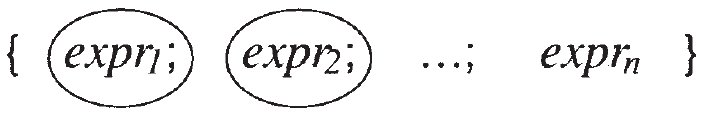
\includegraphics[width=3.2819in,height=0.4736in]{ib-img/ib-img057.jpg}
\end{center}

Note that \textit{exprn }is not, of itself, a bounded expression.
However, it may be part of a larger bounded expression, as in

\begin{center}
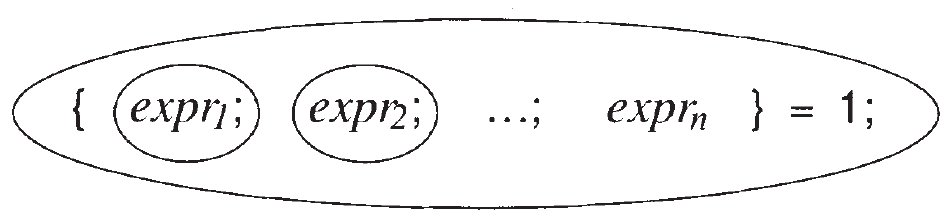
\includegraphics[width=3.5425in,height=0.8173in]{ib-img/ib-img058.jpg}
\end{center}

Here \textit{exprn} is part of the bounded expression for the
comparison operator. The entire enclosing bounded expression is a
consequence of the final semicolon. In the absence of the context
provided by this semicolon, the entire expression might be part of a
larger enclosing bounded expression, and so on.

The separation of a procedure body into a number of bounded
expressions, separated by semicolons (explicit or implicit) and other
syntactic constructions, is very important. Otherwise, a procedure
body would consist of a single expression, and failure of any
component would propagate throughout the entire procedure
body. Instead, control backtracking is limited in scope to abounded
expression, as is the lifetime (and hence stack space) for temporary
computations.

Bounded expressions are particularly important in control
structures. For example, in the if-then-else control structure, the
control expression is bounded but the other expressions are not:

\begin{center}
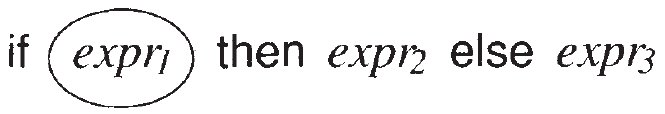
\includegraphics[width=3.5508in,height=0.5244in]{ib-img/ib-img059.jpg}
\end{center}

As with the compound expression illustrated earlier, \textit{expr2} or
\textit{exp13} (whichever is selected) may be the part of a larger
bounded expression. An example is

\begin{center}
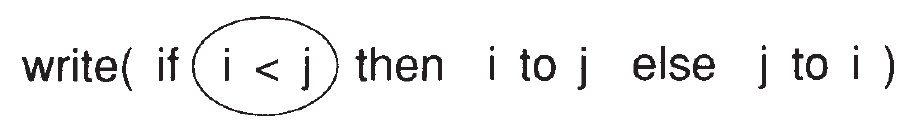
\includegraphics[width=4.0839in,height=0.4571in]{ib-img/ib-img060.jpg}
\end{center}

If the control expression were not a separate bounded expression, the
failure of \textit{expr2} or \textit{exp13} would result in
backtracking into it and the if-then-else expression would be
equivalent to

{\ttfamily\mdseries
\textit{\ \ \ (expr1 }\& \textit{expr2) }{\textbar} \textit{expr3}}

\noindent which is hardly what is meant by if-then-else.

In a while-do loop, the control expression and the expression in the
do clause are both bounded:

\begin{center}
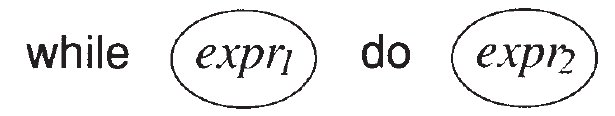
\includegraphics[width=2.8339in,height=0.4992in]{ib-img/ib-img061.jpg}
\end{center}

The two bounded expressions ensure that the expressions are evaluated
independently of each other and any surrounding context. For example,
if \textit{expr2} fails, there is no control backtracking into
\textit{expr}.

\subsection[9.1.1 Expression Frames]{9.1.1 Expression Frames}

In the implementation of Icon, the scope of backtracking is delineated
by \textit{expression frames}. The virtual machine instruction

{\ttfamily\mdseries
\ \ \ mark L1}

\noindent starts an expression frame. If the subsequent expression
fails, \texttt{ipc} is set to the location in the icode that
corresponds to \texttt{L1}. The value of \texttt{ipc} for a label is
relative to the location of the icode that is read in from the icode
file. For simplicity in the description that follows, the value of
\texttt{ipc} is referred to just by the name of the corresponding
label.

The \texttt{mark} instruction pushes an \textit{expression frame
marker }onto the stack and sets the expression frame pointer,
\texttt{efp}, to it. Thus, \texttt{efp} indicates the beginning of the
current expression frame. There is also a generator frame pointer,
\texttt{gfp}, which points to another kind of frame that is used to
retain information when an expression suspends with a result and is
capable of being resumed for another. Generator frames are described
in Sec. 9.3. The mark instruction sets \texttt{gfp} to zero,
indicating that there is no suspended generator in a new expression
frame.

An expression frame marker consists of four words: the value
\texttt{ipc} for the argument of mark (called the failure
\texttt{ipc}), the previous \texttt{efp}, the previous \texttt{gfp},
and \texttt{ilevel}, which is related to suspended generators:


\ \  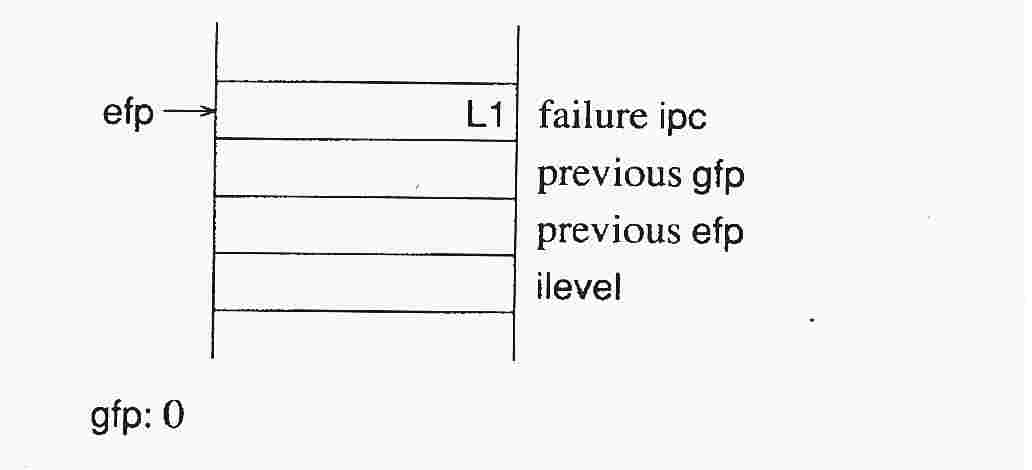
\includegraphics[width=3.5272in,height=1.5689in]{ib-img/ib-img062.jpg} 


An expression frame marker is declared as a C structure:

{\ttfamily\mdseries
\ \ \ struct ef\_marker \{\ \ \ \ /* expression frame marker */}

{\ttfamily\mdseries
\ \ \ \ \ \ word *ef\_failure;\ \ \ \ /*\ \ failure ipc */}

{\ttfamily\mdseries
\ \ \ \ \ \ struct ef\_marker *ef\_efp;\ \ /*\ \ efp */}

{\ttfamily\mdseries
\ \ \ \ \ \ struct gf\_marker *ef\_gfp;\ \ /*\ \ gfp */}

{\ttfamily\mdseries
\ \ \ \ \ \ word ef\_ilevel;\ \ \ \ \ \ /*\ \ ilevel */}


This structure is overlaid on the interpreter stack in order to
reference its components. The code for the \texttt{mark} instruction
is

{\ttfamily\mdseries
\ \ \ case Op\_Mark:\textit{\ \ /* }create expression frame marker \textit{*/}}

{\ttfamily\mdseries
\ \ \ \ \ \ newefp = (struct ef\_marker *)(sp + 1);}

{\ttfamily\mdseries
\ \ \ \ \ \ opnd = GetWord;}

{\ttfamily\mdseries
\ \ \ \ \ \ opnd += (word)ipc;}

{\ttfamily\mdseries
\ \ \ \ \ \ newefp-{\textgreater}ef\_failure = (word *)opnd;}

{\ttfamily\mdseries
\ \ \ \ \ \ newefp-{\textgreater}ef\_gfp = gfp;}

{\ttfamily\mdseries
\ \ \ \ \ \ newefp-{\textgreater}ef\_efp = efp;}

{\ttfamily\mdseries
\ \ \ \ \ \ newefp-{\textgreater}ef\_ilevel = ilevel;}

{\ttfamily\mdseries
\ \ \ \ \ \ sp += Wsizeof(*efp);}

{\ttfamily\mdseries
\ \ \ \ \ \ efp = newefp;}

{\ttfamily\mdseries
\ \ \ \ \ \ gfp = 0;}

{\ttfamily\mdseries
\ \ \ \ \ \ break;}

The macro \texttt{Wsizeof(x)} produces the size of \texttt{x} in words.

An expression frame is removed by the virtual machine instruction

{\ttfamily\mdseries
\ \ \ unmark}

\noindent which restores the previous \texttt{efp} and \texttt{gfp}
from the current expression frame marker and removes the current
expression frame by setting \texttt{sp} to the word just above the
frame marker.

The use of \texttt{mark} and \texttt{unmark} is illustrated by

{\ttfamily\mdseries
\ \ \ if expr1 then \textit{expr2 }else \textit{expr3}}

\noindent for which the virtual machine instructions are

{\ttfamily\mdseries
\ \ \ \ \ \ mark L1}

{\ttfamily\mdseries
\ \ \ \ \ \ code for expr1}

{\ttfamily\mdseries
\ \ \ \ \ \ unmark}

{\ttfamily\mdseries
\ \ \ \ \ \ code for expr2}

{\ttfamily\mdseries
\ \ \ \ \ \ goto L2}

{\ttfamily\mdseries
L1:}

{\ttfamily\mdseries
\ \ \ \ \ \ code for expr3}

{\ttfamily\mdseries
L2:}

The \texttt{mark} instruction creates an expression frame for the
evaluation of \textit{expr1}. If \textit{expr1} produces a result, the
\texttt{unmark} instruction is evaluated, removing the expression
frame for \textit{expr1}, along with the result produced by
\textit{expr1}. Evaluation then proceeds in \textit{expr2}.

If \textit{expr1} fails, control is transferred to the location in the
icode corresponding to \texttt{L1} and the \texttt{unmark} instruction
is not executed. In the absence of generators, failure also removes
the current expression frame, as described in Sec. 9.2.


It is necessary to save the previous value of \texttt{efp} in a new
expression marker, since expression frames may be nested. This occurs
in interesting ways in some generative control structures, which are
discussed in Sec. 9.4. Nested expression frames also occur as a result
of evaluating compound expressions, such as

{\ttfamily\mdseries
\ \ \ while expr1 do ifexpr2thenexpr2}


\section[9.2 Failure]{9.2 Failure}

The interesting aspects of implementing expression evaluation in Icon
can be divided into two cases: without generators and with
generators. The possibility of failure in the absence of generators is
itself of interest, since it occurs in other programming languages,
such as SNOBOL4. This section describes the handling of failure and
assumes, for the moment, that there are no generators. The next
section describes generators.

In the absence of generators, if failure occurs anywhere in an
expression, the entire expression fails without any further
evaluation. For example, in the expressions

{\ttfamily\mdseries
\ \ \ i := numeric(s)}

{\ttfamily\mdseries
\ \ \ line := read(f)}

\noindent if \texttt{numeric(s)} fails in the first line, the
assignment is not performed and evaluation continues immediately with
the second line. In the implementation, this amounts to removing the
current expression frame in which failure occurs and continuing with
\texttt{ipc} set to the failure \texttt{ipc} from its expression frame
marker.

The virtual machine instructions for the previous example are

{\ttfamily\mdseries
\ \ \ mark L1}

{\ttfamily\mdseries
\ \ \ pnull}

{\ttfamily\mdseries
\ \ \ local i}

{\ttfamily\mdseries
\ \ \ global numeric}

{\ttfamily\mdseries
\ \ \ local s}

{\ttfamily\mdseries
\ \ \ invoke 1}

{\ttfamily\mdseries
\ \ \ asgn}

{\ttfamily\mdseries
\ \ \ unmark}

{\ttfamily\mdseries
L1:}

{\ttfamily\mdseries
\ \ \ mark L2}

{\ttfamily\mdseries
\ \ \ pnull}

{\ttfamily\mdseries
\ \ \ local line}

{\ttfamily\mdseries
\ \ \ global read}

{\ttfamily\mdseries
\ \ \ local f}

{\ttfamily\mdseries
\ \ \ invoke 1}

{\ttfamily\mdseries
\ \ \ asgn}

{\ttfamily\mdseries
\ \ \ unmark}

{\ttfamily\mdseries
L2:}

Prior to the evaluation of the expression on the first line, there is
some expression frame on the stack:

\ \  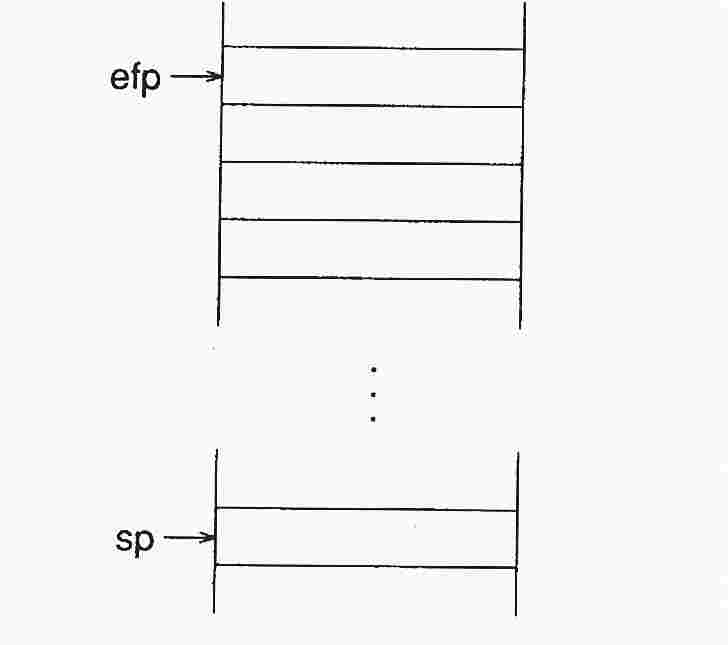
\includegraphics[width=2.4575in,height=2.1543in]{ib-img/ib-img063.jpg} 

The instruction

{\ttfamily\mdseries
\ \ \ mark L1}

\noindent starts a new expression frame. The execution of subsequent
virtual machine instructions pushes additional descriptors.  The state
of the stack when numeric is called by the \texttt{invoke} instruction is

\ \  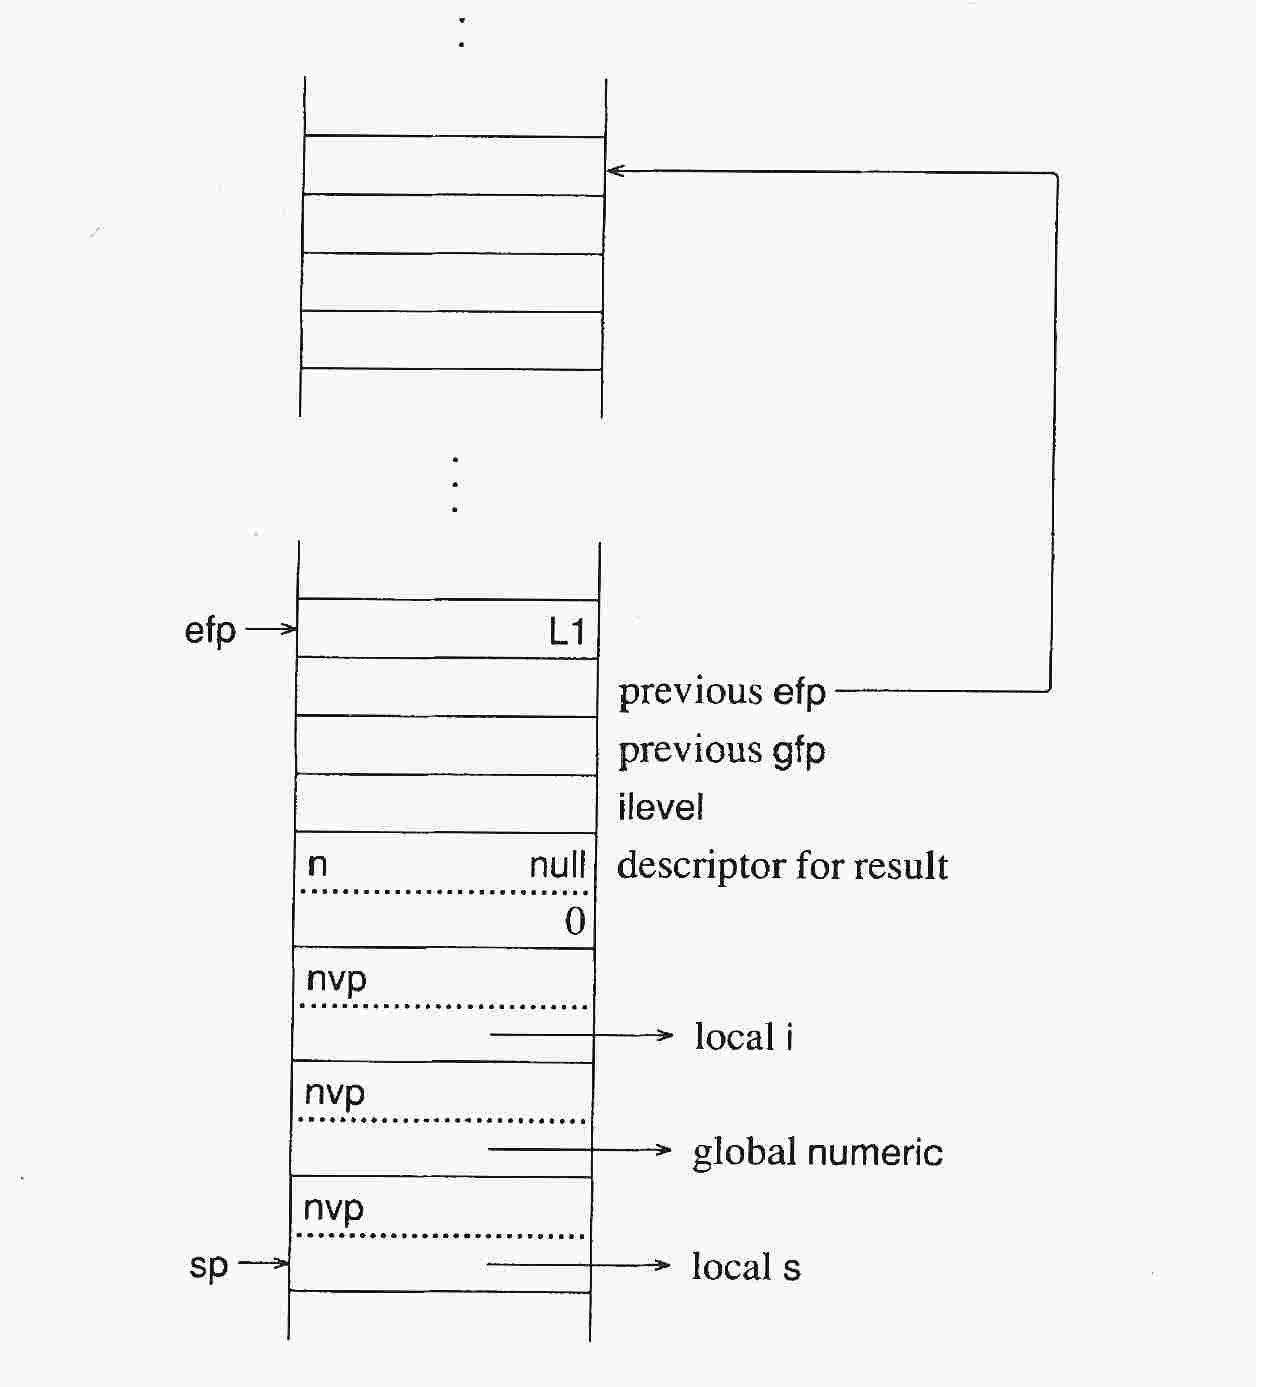
\includegraphics[width=4.2752in,height=4.6319in]{ib-img/ib-img064.jpg} 

If \texttt{numeric(s)} fails, \texttt{efp} and \texttt{sp} are reset,
so that the stack is in the same state as it was prior to the
evaluation of the expression on the first line:

\ \  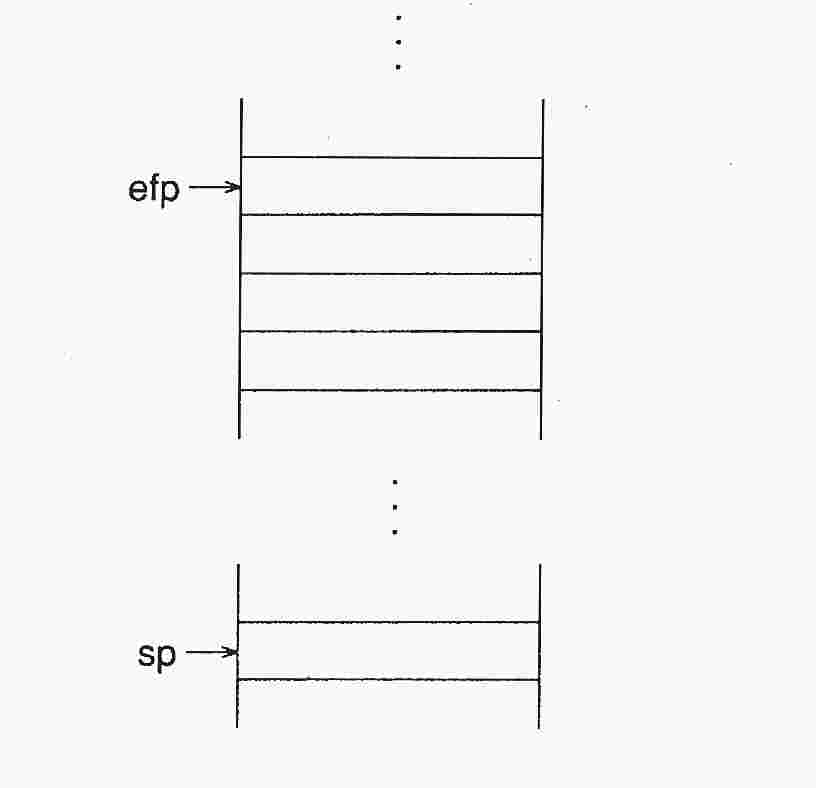
\includegraphics[width=2.778in,height=2.6311in]{ib-img/ib-img065.jpg} 

Control is transferred to the location in the icode corresponding to
\texttt{L1}, and the execution of

{\ttfamily\mdseries
\ \ \ mark L2}

\noindent starts a new expression frame by pushing a new expression
frame marker onto the stack.

It is worth noting that failure causes only the current expression
frame to be removed and changes \texttt{ipc} to the failure
\texttt{ipc}. Any remaining virtual machine instructions in the
current expression frame are bypassed; failure is simple and quick.

Failure can occur at three levels: directly from the virtual machine
instruction \texttt{efail}, from a C function that implements an
operator or function (as in the previous example), or from an Icon
procedure.


When a conditional operator or function returns, it signals the
interpreter, indicating whether it is producing a result or failing by
using one of the RTL forms of return, \texttt{return} or
\texttt{fail}. These RTL constructs simply produce return statements
with different returned values.

The code in the interpreter for a conditional operation is illustrated by

{\ttfamily\mdseries
\ \ \ case Op\_Numlt:\ \ /* e1 {\textless} e2 */}

{\ttfamily\mdseries
\ \ \ \ \ \ Setup\_Op(2);}

{\ttfamily\mdseries
\ \ \ \ \ \ DerefArg(1);}

{\ttfamily\mdseries
\ \ \ \ \ \ DerefArg(2) ;}

{\ttfamily\mdseries
\ \ \ \ \ \ Call\_Cond;}


The macro \texttt{Call\_Cond} is similar to \texttt{Call\_Op}
described in Sec. 8.3.1, but it tests the signal returned by the C
function. If the signal corresponds to the production of a result, the
break is executed and control is transferred to the beginning of the
interpreter loop to fetch the next virtual machine instruction. On the
other hand, if the signal corresponds to failure, control is
transferred to the place in the interpreter that handles failure,
\texttt{efail}.


An Icon procedure can fail in three ways: by evaluating the expression
fail, by the failure of the argument of a return expression, or by
flowing off the end of the procedure body. The virtual machine
instructions generated for the three cases are similar. For example,
the virtual machine instructions for

{\ttfamily\mdseries
\ \ \ if i {\textless} j then fail else write(j)}


are

{\ttfamily\mdseries
\ \ \ mark L1}

{\ttfamily\mdseries
\ \ \ pnull}

{\ttfamily\mdseries
\ \ \ local i}

{\ttfamily\mdseries
\ \ \ local j}

{\ttfamily\mdseries
\ \ \ numlt}

{\ttfamily\mdseries
\ \ \ unmark}

{\ttfamily\mdseries
\ \ \ pfail}

{\ttfamily\mdseries
L1:}

{\ttfamily\mdseries
\ \ \ global write}

{\ttfamily\mdseries
\ \ \ local j}

{\ttfamily\mdseries
\ \ \ invoke 1}

The virtual machine instruction \texttt{pfail} first returns from the
current procedure call (see Sec. 10.3), and then transfers to
\texttt{efail}.


\section[9.3 Generators and Goal{}-Directed Evaluation]{9.3 Generators and Goal-Directed Evaluation}

The capability of an expression not to produce a result is useful for
controlling program flow and for bypassing unneeded computation, but
generators add the real power and expressiveness to the
expression-evaluation semantics of Icon. It should be no surprise that
generators also present difficult implementation problems. There are
several kinds of generators, including those for control structures,
functions and operators, and procedures. While the implementation of
the different kinds of generators varies in detail, the same
principles apply to all of them.


As far as using a result of an expression in further computation is
concerned, there is no difference between an expression that simply
produces a result and an expression that produces a result and is
capable of being resumed to produce mother one. For example, in

{\ttfamily\mdseries
\ \ \ i := numeric({\textquotedbl}2{\textquotedbl})}

{\ttfamily\mdseries
\ \ \ j := upto('aeiou', {\textquotedbl}Hello world{\textquotedbl})}

\noindent the two assignment operations are carried out in the same
way, even though \texttt{upto()} is a generator and \texttt{numeric()}
is not.

Since such contexts cannot be determined, in general, prior to the
time the expressions are evaluated, the implementation is designed so
that the interpreter stack is the same, as far as enclosing
expressions are concerned, whether an expression returns or
suspends. For the previous example, the arguments to the assignment
operation are in the same relative place in both cases.

On the other hand, if a generator that has suspended is resumed, it
must be capable of continuing its computation and possibly producing
another result. For this to be possible, both the generator's state
and the state of the interpreter stack must be preserved. For example,
in

{\ttfamily\mdseries
\ \ \ j := (i {\textless} upto('aeiou', {\textquotedbl}Hello world{\textquotedbl}))}

\noindent when the function \texttt{upto()} suspends, both \texttt{i}
and the result produced by \texttt{upto()} must be on the stack as
arguments of the comparison operation. However, if the comparison
operation fails and \texttt{upto()} is resumed, the arguments of
\texttt{upto()} must be on the stack as they were when \texttt{upto()}
suspended. To satisfy these requirements, when \texttt{upto()}
suspends, a portion of the stack prior to the arguments for
\texttt{upto()} is copied to the top of the stack and the result
produced by upto is placed on the top of the stack. Thus, the portion
of the stack required for the resumption of \texttt{upto()} is
preserved and the arguments for the comparison are in the proper
place.

\textbf{Generator Frames}. When an expression suspends, the state of
the interpreter stack is preserved by creating a \textit{generator
frame} on the interpreter stack that contains a copy of the portion of
the interpreter stack that is needed if the generator is resumed. A
generator frame begins with a generator frame marker that contains
information about the interpreter state that must be restored if the
corresponding generator is resumed. There are three kinds of generator
frames that are distinguished by different codes:


\ \ \ G\_Csusp\ \ suspension from a C function\newline
 \ \ G\_Esusp\ \ suspension from an alternation expression\newline
 \ \ G\_Psusp\ \ suspension from a procedure


For the first two types of generators, the information saved in the
generator frame marker includes the code for the type of the
generator, the i-state variables \texttt{efp}, \texttt{gfp},
\texttt{ipc}, and the source-program line number at the time the
generator frame is created:


\ \  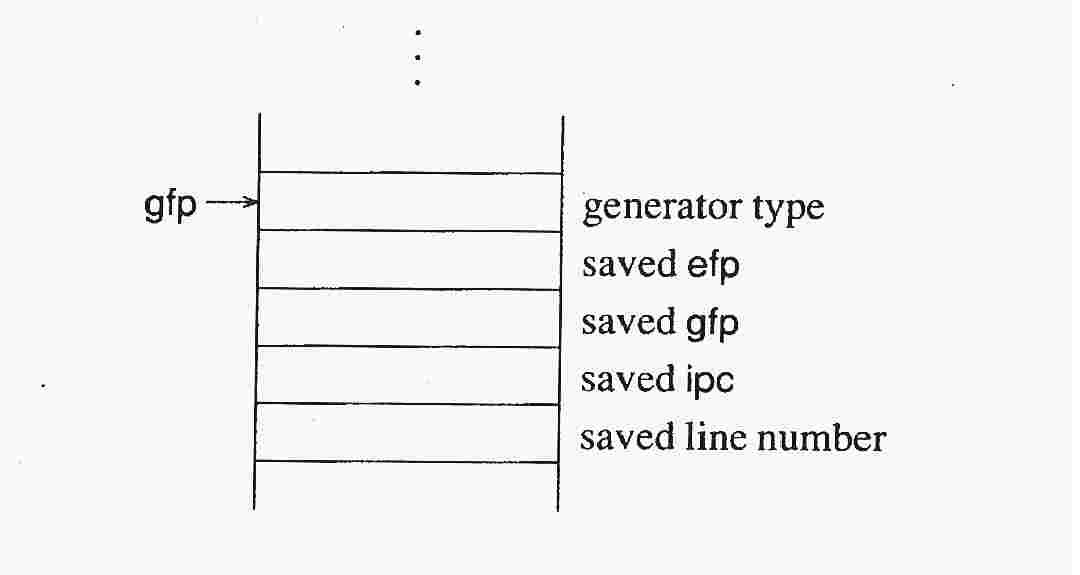
\includegraphics[width=3.6335in,height=1.9193in]{ib-img/ib-img066.jpg} 


The corresponding C structure is

{\ttfamily\mdseries
\ \ \ struct gf\_marker \{\textit{\ \ /* }generator frame marker \textit{*/}}

{\ttfamily\mdseries
\ \ \ \ \ \ word gf\_gentype;\textit{\ \ /*}\ \ type \textit{*/}}

{\ttfamily\mdseries
\ \ \ \ \ \ struct ef\_marker *gf\_efp;\textit{\ \ /*}\ \ efp \textit{*/}}

{\ttfamily\mdseries
\ \ \ \ \ \ struct gf\_marker *gf\_gfp;\textit{\ \ /*}\ \ gfp */}

{\ttfamily\mdseries
\ \ \ \ \ \ word *gf\_ipc;\textit{\ \ /*}\ \ ipc \textit{*/}}

{\ttfamily\mdseries
\ \ \ \ \ \ word gf\_line;\textit{\ \ /*}\ \ line number */}

{\ttfamily\mdseries
\ \ \ \};}


Generators for procedure suspension contain, in addition, the i-state
variable related to procedures. See Sec. 10.3.3.

As an example, consider the expression

{\ttfamily\mdseries
\ \ \ write(i = (1 to 3));}


The virtual machine instructions for this expression are:

{\ttfamily\mdseries
\ \ \ mark L1}

{\ttfamily\mdseries
\ \ \ global write}

{\ttfamily\mdseries
\ \ \ pnull}

{\ttfamily\mdseries
\ \ \ local i}

{\ttfamily\mdseries
\ \ \ int 1}

{\ttfamily\mdseries
\ \ \ int 3}

{\ttfamily\mdseries
\ \ \ push 1\ \ \# default increment}

{\ttfamily\mdseries
\ \ \ toby}

{\ttfamily\mdseries
\ \ \ numeq}

{\ttfamily\mdseries
\ \ \ invoke 1}

{\ttfamily\mdseries
\ \ \ unmark}

{\ttfamily\mdseries
L1 :}


The state of the stack after execution of the first seven instructions is


\ \  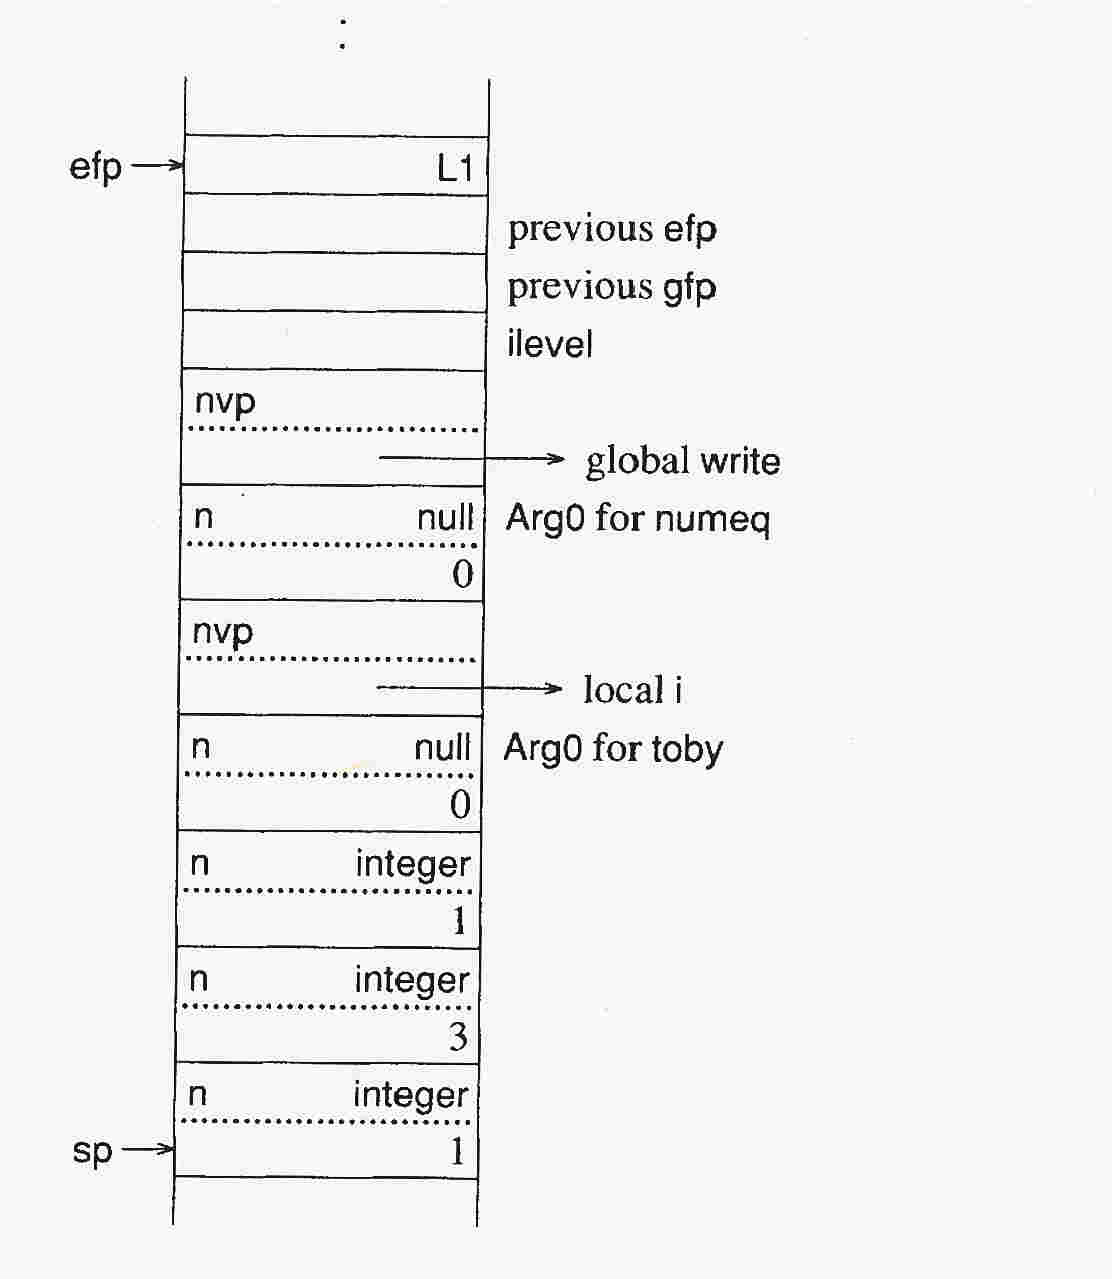
\includegraphics[width=3.7402in,height=4.2717in]{ib-img/ib-img067.jpg} 


The code in the interpreter for calling a generative operator with n
arguments is

{\ttfamily\mdseries
\ \ \ rargp = (struct descrip *)(sp -1) -n;}

{\ttfamily\mdseries
\ \ \ signal = (*(optab[op]))(rargp);}

{\ttfamily\mdseries
\ \ \ goto C\_rtn\_term;}


Note that \texttt{rargp} points to Arg0 and is the argument of the
call to the C function for the operator.

The RTL function for \texttt{toby} is

{\ttfamily\mdseries
operator\{*\} ... toby(from, to, by)}

{\ttfamily\mdseries
\ \ \ /*}

{\ttfamily\mdseries
\ \ \ \ * arguments must be integers.}

{\ttfamily\mdseries
\ \ \ \ */}

{\ttfamily\mdseries
\ \ \ if !cnv:C\_integer(from) then}

{\ttfamily\mdseries
\ \ \ \ \ \ runerr(101, from)}

{\ttfamily\mdseries
\ \ \ if !cnv:C\_integer(to) then}

{\ttfamily\mdseries
\ \ \ \ \ \ runerr(101, to)}

{\ttfamily\mdseries
\ \ \ if !cnv:C\_integer(by) then}

{\ttfamily\mdseries
\ \ \ \ \ \ runerr(101, by)}

{\ttfamily\mdseries
\ \ \ abstract \{}

{\ttfamily\mdseries
\ \ \ \ \ \ return integer}

{\ttfamily\mdseries
\ \ \ \ \ \ \}}

{\ttfamily\mdseries
\ \ \ inline \{}

{\ttfamily\mdseries
\ \ \ \ \ \ /*}

{\ttfamily\mdseries
\ \ \ \ \ \ \ * by must not be zero.}

{\ttfamily\mdseries
\ \ \ \ \ \ \ */}

{\ttfamily\mdseries
\ \ \ \ \ \ if (by == 0) \{}

{\ttfamily\mdseries
\ \ \ \ \ \ \ \ \ irunerr(211, by);}

{\ttfamily\mdseries
\ \ \ \ \ \ \ \ \ errorfail;}

{\ttfamily\mdseries
\ \ \ \ \ \ \ \ \ \}}

{\ttfamily\mdseries
\ \ \ \ \ \ /*}

{\ttfamily\mdseries
\ \ \ \ \ \ \ * Count up or down (depending on relationship of from and}

{\ttfamily\mdseries
\ \ \ \ \ \ \ * \ to) and suspend each value in sequence, failing when}

{\ttfamily\mdseries
\ \ \ \ \ \ \ * \ the limit has been exceeded.}

{\ttfamily\mdseries
\ \ \ \ \ \ \ */}

{\ttfamily\mdseries
\ \ \ \ \ \ if (by {\textgreater} 0)}

{\ttfamily\mdseries
\ \ \ \ \ \ \ \ \ for ( ; from {\textless}= to; from += by) \{}

{\ttfamily\mdseries
\ \ \ \ \ \ \ \ \ \ \ \ suspend C\_integer from;}

{\ttfamily\mdseries
\ \ \ \ \ \ \ \ \ \ \ \ \}}

{\ttfamily\mdseries
\ \ \ \ \ \ else}

{\ttfamily\mdseries
\ \ \ \ \ \ \ \ \ for ( ; from {\textgreater}= to; from += by) \{}

{\ttfamily\mdseries
\ \ \ \ \ \ \ \ \ \ \ \ suspend C\_integer from;}

{\ttfamily\mdseries
\ \ \ \ \ \ \ \ \ \ \ \ \}}

{\ttfamily\mdseries
\ \ \ \ \ \ fail;}

{\ttfamily\mdseries
\ \ \ \ \ \ \}}

{\ttfamily\mdseries
end}

The RTL \texttt{operator} construct, which is similar to
\texttt{function}, produces the C header

{\ttfamily\mdseries
int Otoby(dptr r\_args)}

\noindent so that \texttt{toby} is called with a pointer to
Arg0. Arguments with logical names Arg0, Arg1, and so forth are
referred as \texttt{r\_args[0]}, \texttt{r\_args[1]}, and so on in the
generated code.

When \texttt{toby} is called, it replaces its Arg0 descriptor by a
descriptor for the integer \texttt{from} and suspends by using the RTL
\texttt{suspend} construct rather than \texttt{return}.

The \texttt{suspend} statement \textit{calls }\texttt{interp()}
instead of returning to it. This leaves the call of \texttt{toby}
intact with its variables preserved and also transfers control to
\texttt{interp()} so that the next virtual machine instruction can be
interpreted. However, it is necessary to push a generator marker on
the interpreter stack and copy a portion of the interpreter stack, so
that interpretation can continue without changing the portion of the
interpreter stack that \texttt{toby} needs in case it is resumed. This
is accomplished by calling \texttt{interp()} with arguments that
signal it to build a generator frame. The C code generated for
\texttt{suspend} is

{\ttfamily\mdseries
\ \ \ if ((signal = interp(G\_Osusp, r\_args RTTCURTSTATARG)) !=}

{\ttfamily\mdseries
\ \ \ \ \ \ \ \ A\_Resume) \{}

{\ttfamily\mdseries
\ \ \ \ \ \ return signal;}

{\ttfamily\mdseries
\ \ \ \ \ \ \}}

The argument \texttt{G\_Osusp} in the call of \texttt{interp()}
indicates that a generator frame for C function that implements an
operator is needed. The argument \texttt{r\_args} points to the
location on the interpreter stack where Arg0 for the suspending C
function is located. This location is the same as rargp in the call of
\texttt{interp()} that called upto.

In this situation, \texttt{interp()} puts a generator frame marker on
the interpreter stack and copies the portion of the interpreter stack
from the last expression 01 generator frame marker through cargp onto
the top of the interpreter stack:

\ \  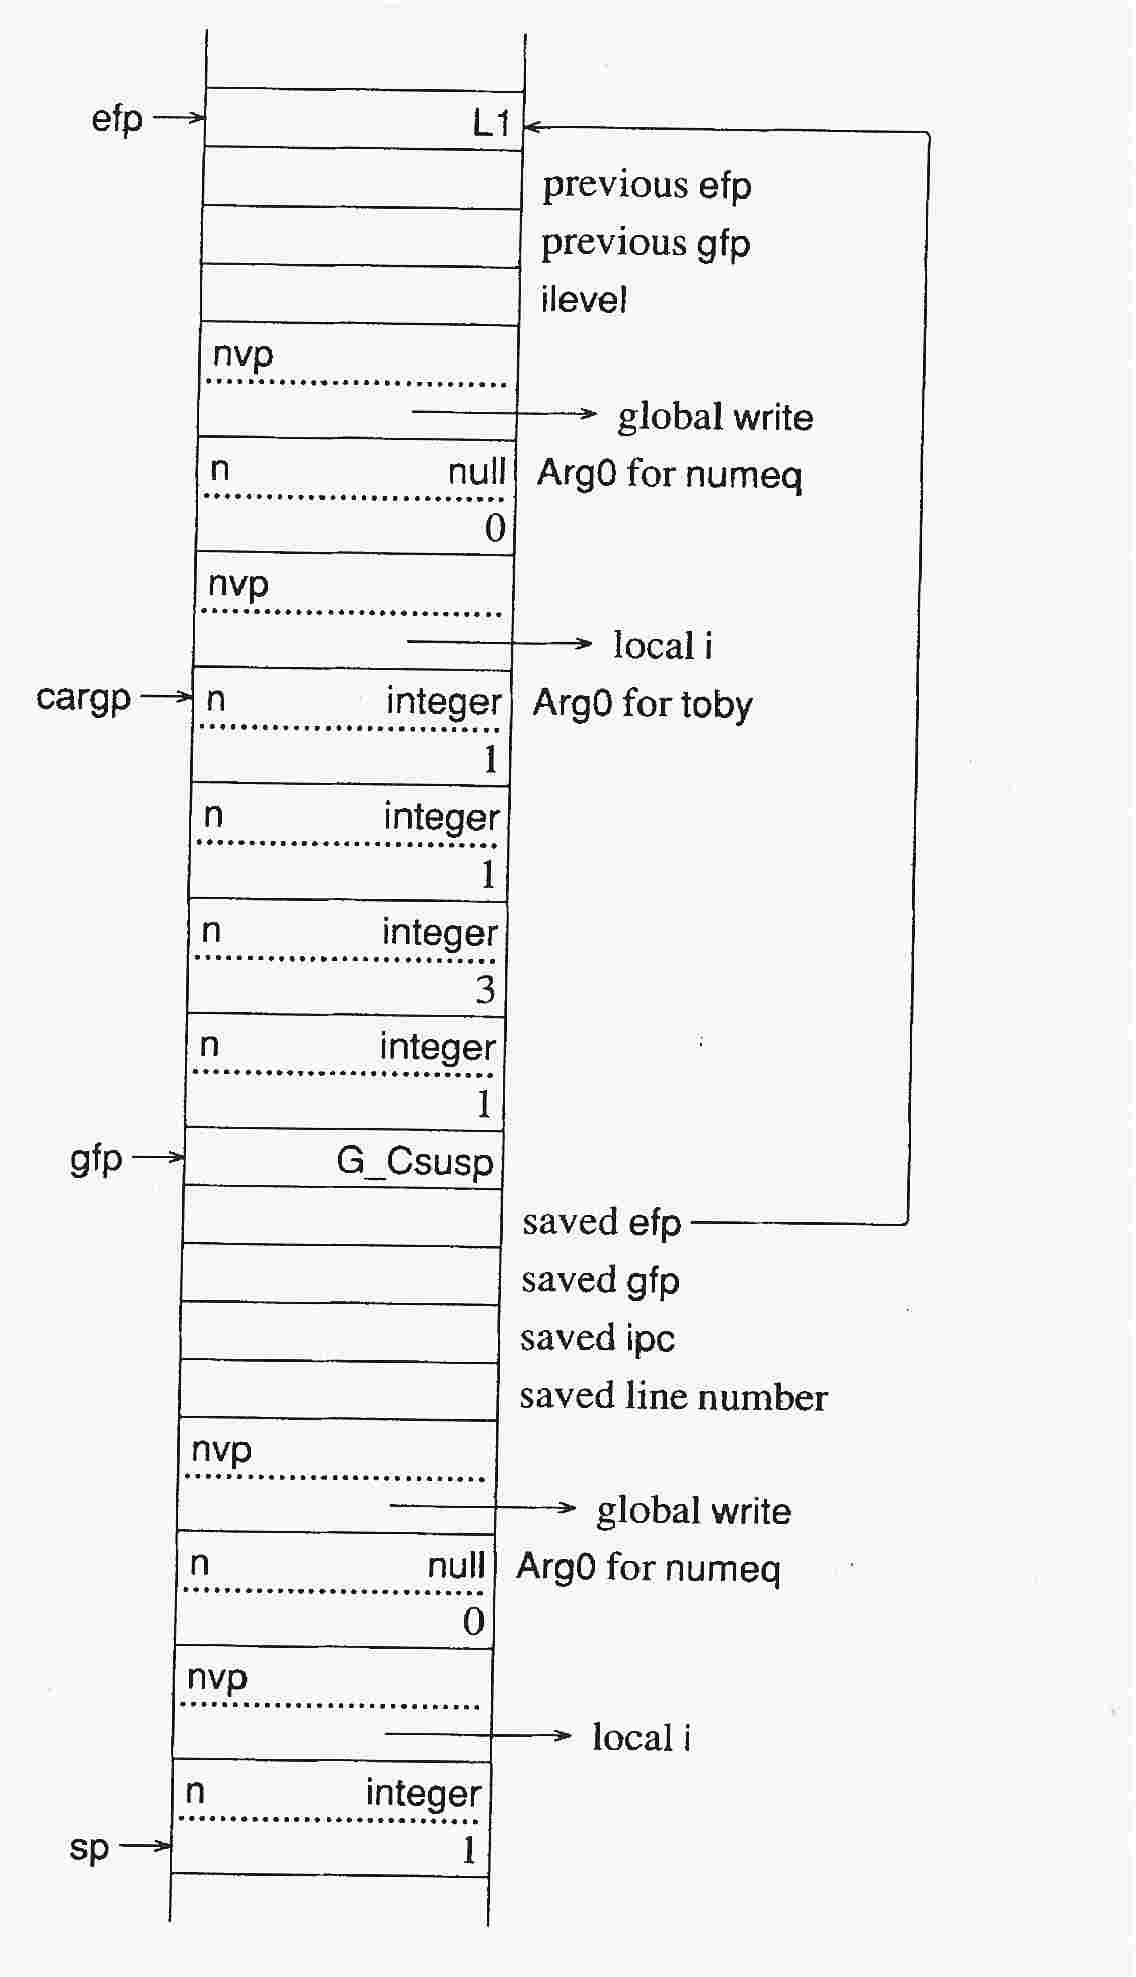
\includegraphics[width=3.848in,height=6.6035in]{ib-img/ib-img068.jpg} 

The stack is exactly the same, as far as the execution of
\texttt{numeq} is concerned, as it would have been if \texttt{toby}
had simply returned. However, the arguments of \texttt{toby} (and the
\ preceding arguments of \texttt{numeq}) are still intact, so that
\texttt{toby} can be resumed. The generator frame is interposed
between the two portions of the interpreter stack. The top of the
stack corresponds to the evaluation of

{\ttfamily\mdseries
\ \ \ write(i = 1);}


\textbf{Resumption}.\ \ Suppose the value of \texttt{i} in the
previous example is 2. The comparison fails and control is transferred
to \texttt{efail}, as it is in the case of all operations that
fail. The code for \texttt{efail} is

{\ttfamily\mdseries
\ \ \ case Op\_Efail:}

{\ttfamily\mdseries
\ \ \ efail:}

{\ttfamily\mdseries
\ \ \ \ \ \ /*}

{\ttfamily\mdseries
\ \ \ \ \ \ \ * Failure has occurred in the current expression frame.}

{\ttfamily\mdseries
\ \ \ \ \ \ \ */}

{\ttfamily\mdseries
\ \ \ \ \ \ if (gfp == 0) \{}

{\ttfamily\mdseries
\ \ \ \ \ \ \ \ \ /*}

{\ttfamily\mdseries
\ \ \ \ \ \ \ \ \ \ * There are no suspended generators to resume. Remove}

{\ttfamily\mdseries
\ \ \ \ \ \ \ \ \ \ * the current expression frame, restoring values.}

{\ttfamily\mdseries
\ \ \ \ \ \ \ \ \ \ *}

{\ttfamily\mdseries
\ \ \ \ \ \ \ \ \ \ * If the failure ipc is 0, propagate failure to the}

{\ttfamily\mdseries
\ \ \ \ \ \ \ \ \ \ * enclosing frame by branching back to efail.}

{\ttfamily\mdseries
\ \ \ \ \ \ \ \ \ \ * This happens, for example, in looping control}

{\ttfamily\mdseries
\ \ \ \ \ \ \ \ \ \ * structures that fail when complete.}

{\ttfamily\mdseries
\ \ \ \ \ \ \ \ \ \ */}

{\ttfamily\mdseries
\ \ \ \ \ \ \ \ \ ipc = efp-{\textgreater}ef\_failure;}

{\ttfamily\mdseries
\ \ \ \ \ \ \ \ \ gfp = efp-{\textgreater}ef-9fp;}

{\ttfamily\mdseries
\ \ \ \ \ \ \ \ \ sp = (word *)efp -1;}

{\ttfamily\mdseries
\ \ \ \ \ \ \ \ \ efp = efp-{\textgreater}ef\_efp;}

{\ttfamily\mdseries
\ \ \ \ \ \ \ \ \ if (ipc == 0)}

{\ttfamily\mdseries
\ \ \ \ \ \ \ \ \ \ \ \ goto efail;}

{\ttfamily\mdseries
\ \ \ \ \ \ \ \ \ break;}

{\ttfamily\mdseries
\ \ \ \ \ \ \ \ \ \}}

{\ttfamily\mdseries
\ \ \ \ \ \ else \{}

{\ttfamily\mdseries
\ \ \ \ \ \ \ \ \ /*}

{\ttfamily\mdseries
\ \ \ \ \ \ \ \ \ \ * There is a, generator that can be resumed. Make}

{\ttfamily\mdseries
\ \ \ \ \ \ \ \ \ \ * the stack adjustments and then switch on the}

{\ttfamily\mdseries
\ \ \ \ \ \ \ \ \ \ * type of the generator frame marker.}

{\ttfamily\mdseries
\ \ \ \ \ \ \ \ \ \ */}

{\ttfamily\mdseries
\ \ \ \ \ \ \ \ \ register struct gf\_marker *resgfp = gfp;}

{\ttfamily\mdseries
\ \ \ \ \ \ \ \ \ tvoe = resgfp-{\textgreater}gf gentype;}

{\ttfamily\mdseries
\ \ \ \ \ \ \ \ \ ipc = resgfp-{\textgreater}gf\_ipc;}

{\ttfamily\mdseries
\ \ \ \ \ \ \ \ \ efp = resgfp-{\textgreater}gf\_efp;}

{\ttfamily\mdseries
\ \ \ \ \ \ \ \ \ line = resgfp-{\textgreater}gf\_line;}

{\ttfamily\mdseries
\ \ \ \ \ \ \ \ \ gfp = resgfp-{\textgreater}gf\_gfp;}

{\ttfamily\mdseries
\ \ \ \ \ \ \ \ \ sp = (word * )resgfp -1;}

{\ttfamily\mdseries
\ \ \ \ \ \ \ \ \ switch (type) \{}


\ \ \ \ \ \ \ \ \ case G\_Csusp: \{


\ \ \ \ \ \ \ \ \ \ \ \ {}-{}-ilevel;

{\ttfamily\mdseries
\ \ \ \ \ \ \ \ \ \ \ \ return A\_Resumption;}

{\ttfamily\mdseries
\ \ \ \ \ \ \ \ \ \ \ \ \textrm{break;}}

{\ttfamily\mdseries
\ \ \ \ \ \ \ \ \ \ \ \ \}}

{\ttfamily\mdseries
\ \ \ \ \ \ \ \ \ case G\_Esusp:}

{\ttfamily\mdseries
\ \ \ \ \ \ \ \ \ \ \ \ goto efail;}

{\ttfamily\mdseries
\ \ \ \ \ \ \ \ \ case G\_Psusp:}

{\ttfamily\mdseries
\ \ \ \ \ \ \ \ \ \ \ \ break;}

{\ttfamily\mdseries
\ \ \ \ \ \ \ \ \ \}}

{\ttfamily\mdseries
\ \ \ \ \ \ break;}

{\ttfamily\mdseries
\ \ \ \ \ \ \}}


If there were no generator frame (if \texttt{gfp} were 0), the entire
expression frame would be removed, and the expression would fail as
described in Sec. 9.2. However, since there is a C\_Susp generator
frame, the stack is restored to the state it\ \ is in when
\texttt{toby} suspended, and the values saved in the generator frame
marker are \textit{restored:}


\ \  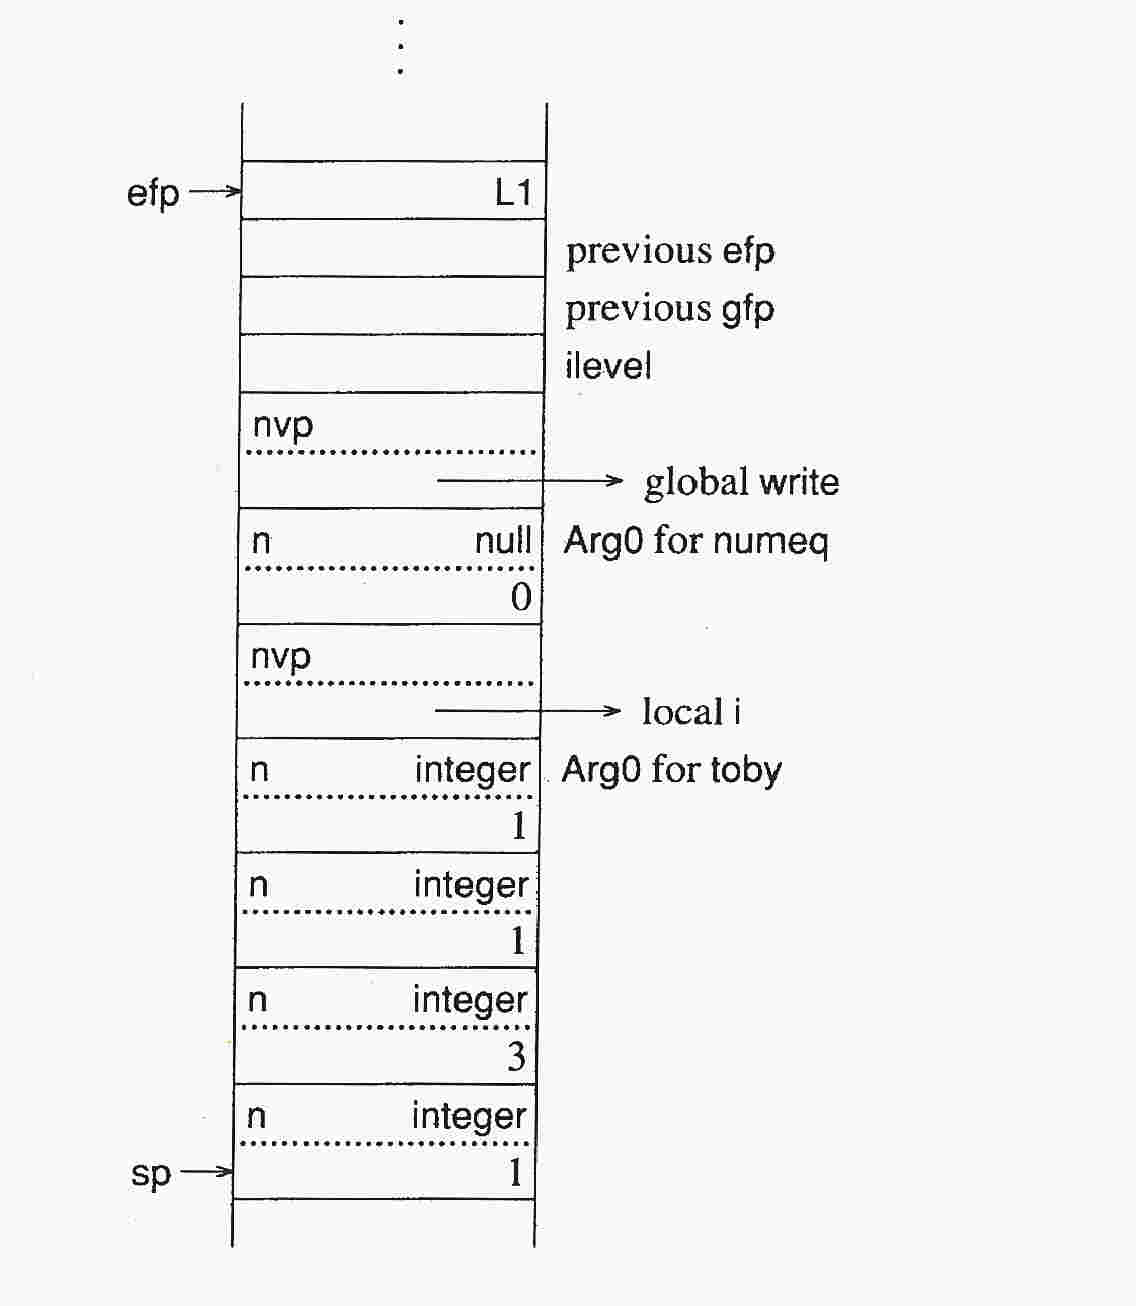
\includegraphics[width=3.848in,height=4.361in]{ib-img/ib-img069.jpg} 


All traces of the first execution of \texttt{numeq} have been removed
from the stack. As shown by the code for \texttt{efail}, the call to
\texttt{toby} is resumed by \textit{returning} to it from
\texttt{interp()} with the signal \texttt{A\_Resumption}, which
indicates another result is needed. When control is returned to
\texttt{toby}, it changes its Arg0 descriptor to the integer 2
suspends again:


\ \  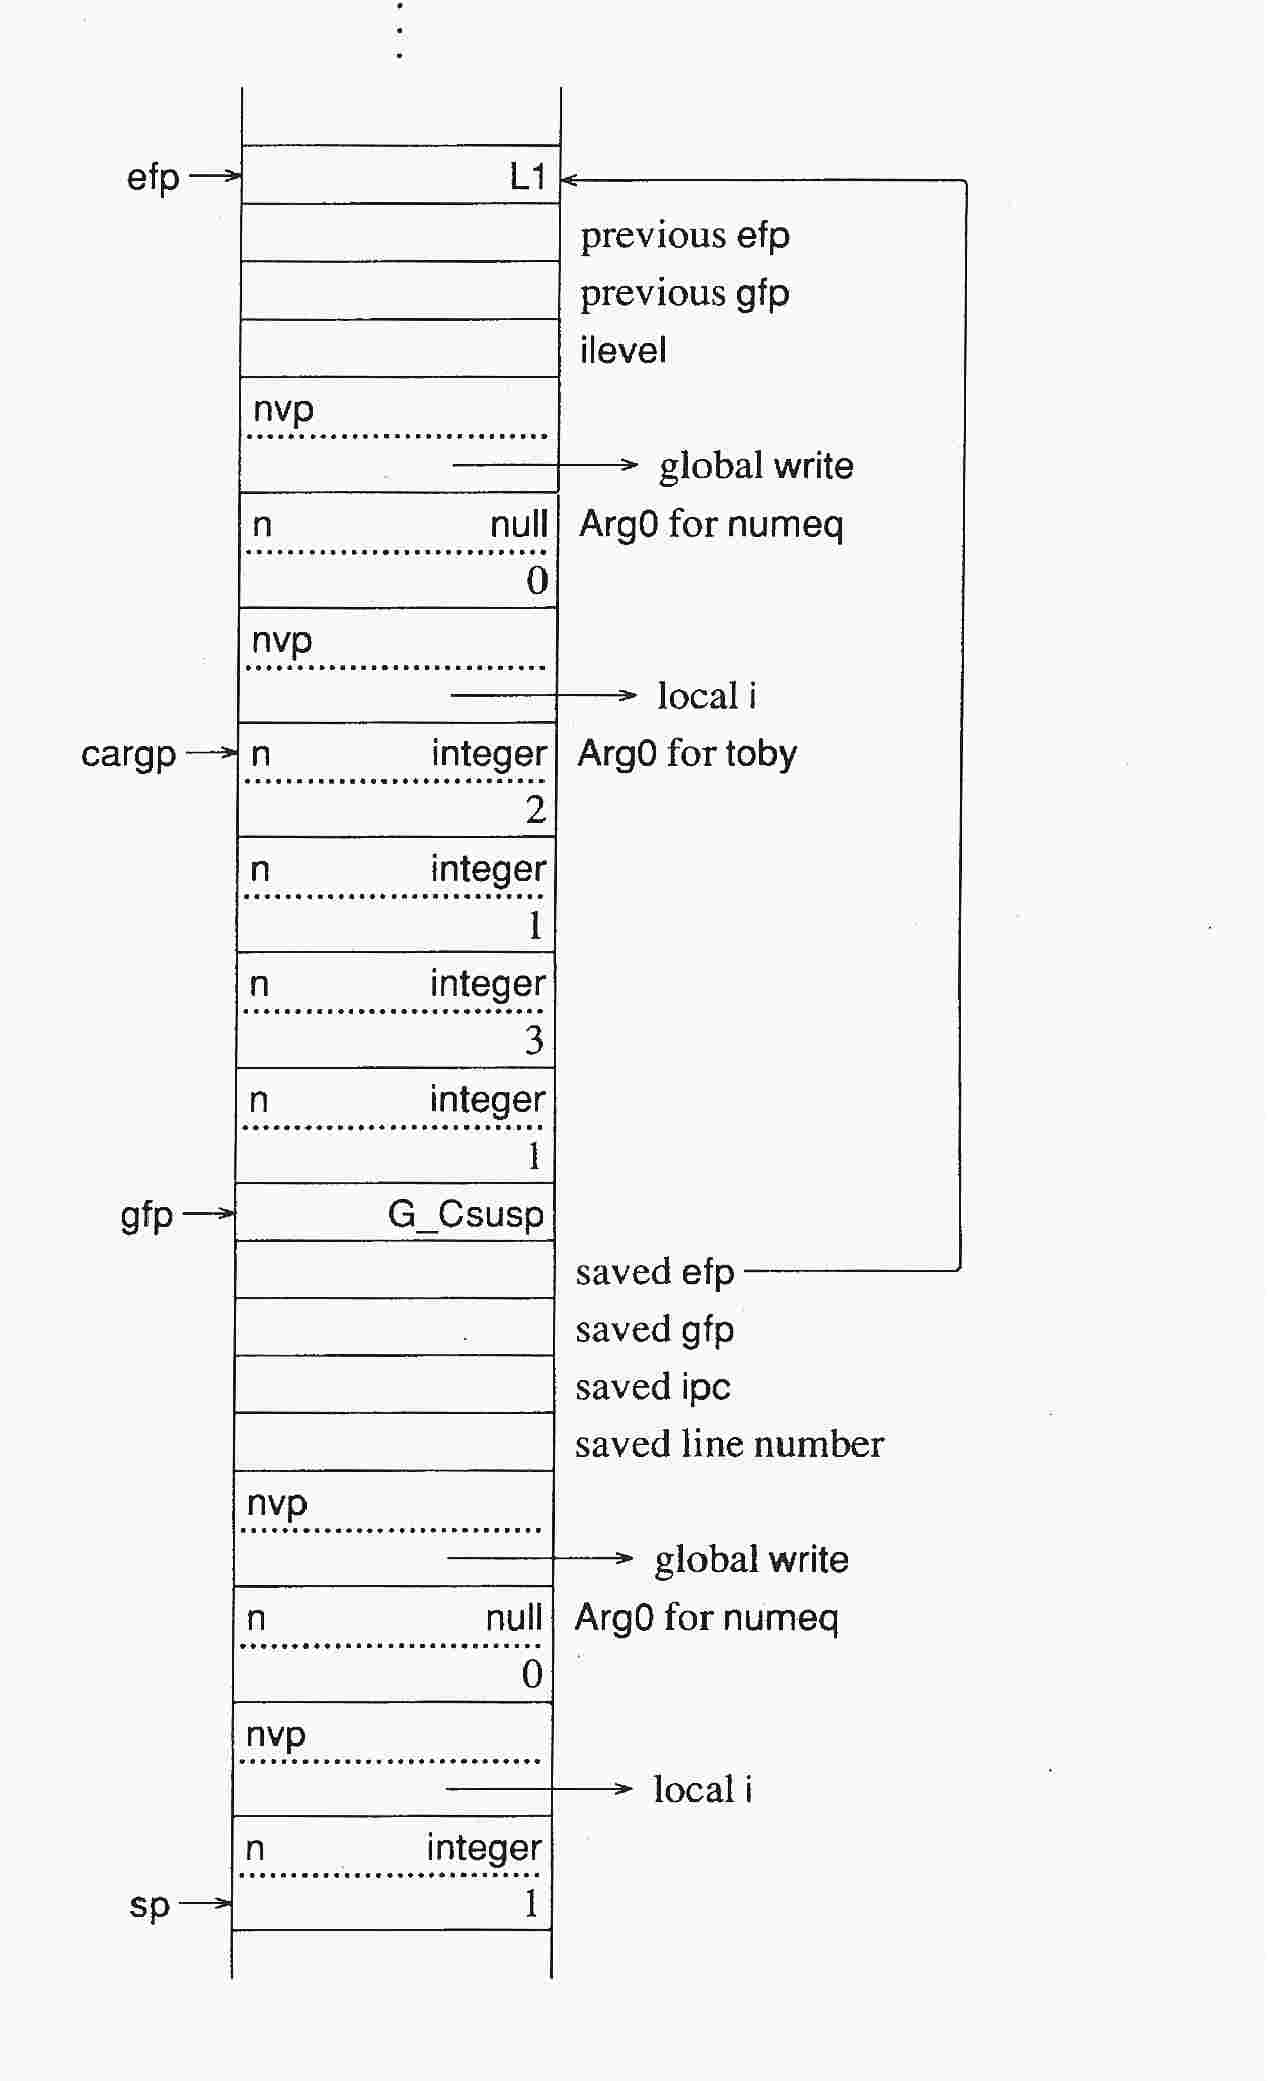
\includegraphics[width=4.2752in,height=6.9508in]{ib-img/ib-img070.jpg} 


The interpreter stack is exactly as it was when \texttt{toby}
suspended the first time, except that the integer 2 is on the stack in
place of the integer 1. The top of the stack corresponds to the
evaluation of

{\ttfamily\mdseries
\ \ \ write(i = 2);}


Since the value of \texttt{i} is 2, \texttt{numeq} succeeds. It copies
the value of its second argument to its Arg0 descriptor and
returns. The value 2 is written and the \texttt{unmark} instruction is
executed, removing the entire expression frame from the stack.


\textbf{Goal-Directed Evaluation. }Goal-directed evaluation occurs
when an expression fails and there are generator frames on the
interpreter stack as the consequence of expressions that have
suspended.

In the case of an expression such as

{\ttfamily\mdseries
\ \ \ 1 to upto(c, s)}

\noindent \texttt{upto()} suspends first, followed by
\texttt{toby}. These generator frames are linked together, with
\texttt{gfp} pointing to the one for \texttt{toby}, which in turn
contains a pointer to the one for \texttt{upto()}. In general,
generator frames are linked together with \texttt{gfp} pointing to the
one for the most recent suspension. This produces the last-in,
first-out (depth-first) \textit{order of} expression evaluation in
Icon. Goal-directed evaluation occurs as a result of resuming
a suspended expression when failure occurs in the surrounding
expression frame.


\textbf{Removing C Frames.} Since C functions that suspend call the
interpreter and the interpreter in turn calls C functions, expression
evaluation typically results in a sequence of frames for calls on the
C stack. When the evaluation of a bounded expression is complete,
there may be frames on the C stack for generators, even though these
generators no longer can be resumed.

In order to {\textquotedbl}unwind{\textquotedbl} the C stack in such
cases, the i-state variable \texttt{ilevel} is used to keep track of
the level of call of \texttt{interp()} by C functions. Whenever
\texttt{interp()} is called, it increments \texttt{ilevel}. When an
expression frame is created, the current value of \texttt{ilevel} is
saved in it, as illustrated previously.

When the expression frame is about to be removed, if the current value
of \texttt{ilevel} is greater than the value in the current expression
frame, \texttt{ilevel} is decremented and the interpreter
\textit{returns }with a signal to the C function that called it to
return rather than to produce another result. If the signal returned
by \texttt{interp()} is \texttt{A\_Resumption}, the C function
continues execution, while for any other signal the C function
returns.

Since C functions return to \texttt{interp()}, \texttt{interp()}
always checks the signal returned to it to determine if it produced a
result or if it is unwinding. If it is unwinding, \texttt{interp()}
returns the unwinding signal instead of continuing evaluation
of\textit{ }the current expression.

Consider again the expression

{\ttfamily\mdseries
\ \ \ write(i = (1 to 3));}

\noindent for which the virtua1 machine instructions are

{\ttfamily\mdseries
\ \ \ mark L1}

{\ttfamily\mdseries
\ \ \ global write}

{\ttfamily\mdseries
\ \ \ pnull}

{\ttfamily\mdseries
\ \ \ local i}

{\ttfamily\mdseries
\ \ \ int 1}

{\ttfamily\mdseries
\ \ \ int 3}

{\ttfamily\mdseries
\ \ \ push1\ \ \# default increment}

{\ttfamily\mdseries
\ \ \ toby}

{\ttfamily\mdseries
\ \ \ numeq}

{\ttfamily\mdseries
\ \ \ invoke 1}

{\ttfamily\mdseries
\ \ \ unmark}

{\ttfamily\mdseries
L1 :}


When \texttt{toby} produces a result, it calls \texttt{interp()}. When
the \texttt{unmark} instruction is executed, the C stack contains a
frame for the call to \texttt{toby} and for its call to
\texttt{interp()}. The code for \texttt{unmark} is

{\ttfamily\mdseries
\ \ \ case Op\_Unmark:\ \ /* remove expression frame */}

{\ttfamily\mdseries
\ \ \ \ \ \ gfp = efp-{\textgreater}ef-9fp;}

{\ttfamily\mdseries
\ \ \ \ \ \ sp = (word *)efp -1;}

{\ttfamily\mdseries
\ \ \ \ \ \ /*}

{\ttfamily\mdseries
\ \ \ \ \ \ \ * Remove any suspended C generators.}

{\ttfamily\mdseries
\ \ \ \ \ \ \ */}

{\ttfamily\mdseries
\ \ \ Unmark\_uw:}

{\ttfamily\mdseries
\ \ \ \ \ \ if (efp-{\textgreater}ef\_ilevel {\textless} ilevel) \{}

{\ttfamily\mdseries
\ \ \ \ \ \ \ \ \ {}-{}-ilevel;}

{\ttfamily\mdseries
\ \ \ \ \ \ \ \ \ return A\_Unmark\_uw;}

{\ttfamily\mdseries
\ \ \ \ \ \ \ \ \ \}}

{\ttfamily\mdseries
\ \ \ \ \ \ efp = efp-{\textgreater}ef\_efp;}

{\ttfamily\mdseries
\ \ \ \ \ \ break;}

Note that in this case Suspend gets the return code
\texttt{A\_Unmark\_uw} and in turn returns \texttt{A\_Unmark\_uw} to
\texttt{interp()}. The section of code in \texttt{interp()} that
checks the signal that is returned from C functions is

{\ttfamily\mdseries
\ \ \ C\_rtn\_term:}

{\ttfamily\mdseries
\ \ \ \ \ \ switch (signal) \{}

{\ttfamily\mdseries
\ \ \ \ \ \ case A\_Failure:}

{\ttfamily\mdseries
\ \ \ \ \ \ \ \ \ goto efail;}

{\ttfamily\mdseries
\ \ \ \ \ \ case A\_Unmark\_uw:\ \ /* unwind for unmark */}

{\ttfamily\mdseries
\ \ \ \ \ \ \ \ \ goto Unmark uw;}

{\ttfamily\mdseries
\ \ \ \ \ \ case A\_Lsusp\_uw:\ \ /* unwind for Isusp */}

{\ttfamily\mdseries
\ \ \ \ \ \ \ \ \ goto Lsusp\_uw;}

{\ttfamily\mdseries
\ \ \ \ \ \ case A\_Eret\_uw:\ \ /* unwind for eret */}

{\ttfamily\mdseries
\ \ \ \ \ \ \ \ \ goto Eret\_uw;}

{\ttfamily\mdseries
\ \ \ \ \ \ case A\_Pret\_uw:\ \ /* unwind for pret */}

{\ttfamily\mdseries
\ \ \ \ \ \ \ \ \ goto Pret\_uw;}

{\ttfamily\mdseries
\ \ \ \ \ \ case A\_Pfail\_uw:\ \ /* unwind for pfail */}

{\ttfamily\mdseries
\ \ \ \ \ \ \ \ \ goto Pfail\_uw;}

{\ttfamily\mdseries
\ \ \ \ \ \ \}}

{\ttfamily\mdseries
\ \ \ \ \ \ sp = (word * )rargp + 1;\ \ /* set sp to result */}

{\ttfamily\mdseries
\ \ \ \ \ \ continue;}

{\ttfamily\mdseries
\ \ \ \}}


Thus, when \texttt{interp()} returns to a C function with an unwinding
signal, there is a cascade of C returns until \texttt{ilevel} is the
same as it was when the current expression frame was created. Note
that there are several cases in addition to \texttt{unmark} where
unwinding is necessary.

\section[9.4 Generative Control Structures]{9.4 Generative Control Structures}

In addition to functions and operators that may generate more than one
result, there are several generative control structures at the level
of virtual machine instructions.

\subsection[9.4.1 Alternation]{9.4.1 Alternation}

The virtual machine instructions for

{\ttfamily\mdseries
\ \ \ \ \ \ \textit{expr\TextSubscript{2}} {\textbar} \textit{expr\TextSubscript{3}}}

are

{\ttfamily\mdseries
\ \ \ mark L1}

{\ttfamily\itshape
\ \ \ code for expr\TextSubscript{2}}


\textit{\ \ \ }esusp

{\ttfamily\mdseries
\ \ \ goto L2}

{\ttfamily\mdseries
L1:}

{\ttfamily\mdseries
\ \ \ \textit{code for expr}\textit{\TextSubscript{3}}}

{\ttfamily\mdseries
L2:}


The mark instruction creates an expression frame marker for
alternation whose purpose is to preserve the failure \texttt{ipc} for
\texttt{L1} in case the results for \textit{expr3 }are needed. If
\textit{expr2 }produces a result, \texttt{esusp} creates a generator
frame with the usual marker and then copies the portion of the
interpreter stack between the last expression or generator frame
marker and the alternation marker to the top of the stack. It then
pushes a copy of the result produced by \textit{expr2}. This connects
the result produced by \textit{expr2 }with the expression prior to the
alternation control structure. Next, \texttt{esusp} sets \texttt{efp}
to point to the expression frame marker prior to the alternation
marker. For example, in the expression

{\ttfamily\mdseries
\ \ \ write(i := 1 {\textbar} 2)}

\noindent the stack after the execution of \texttt{esusp} is


\ \  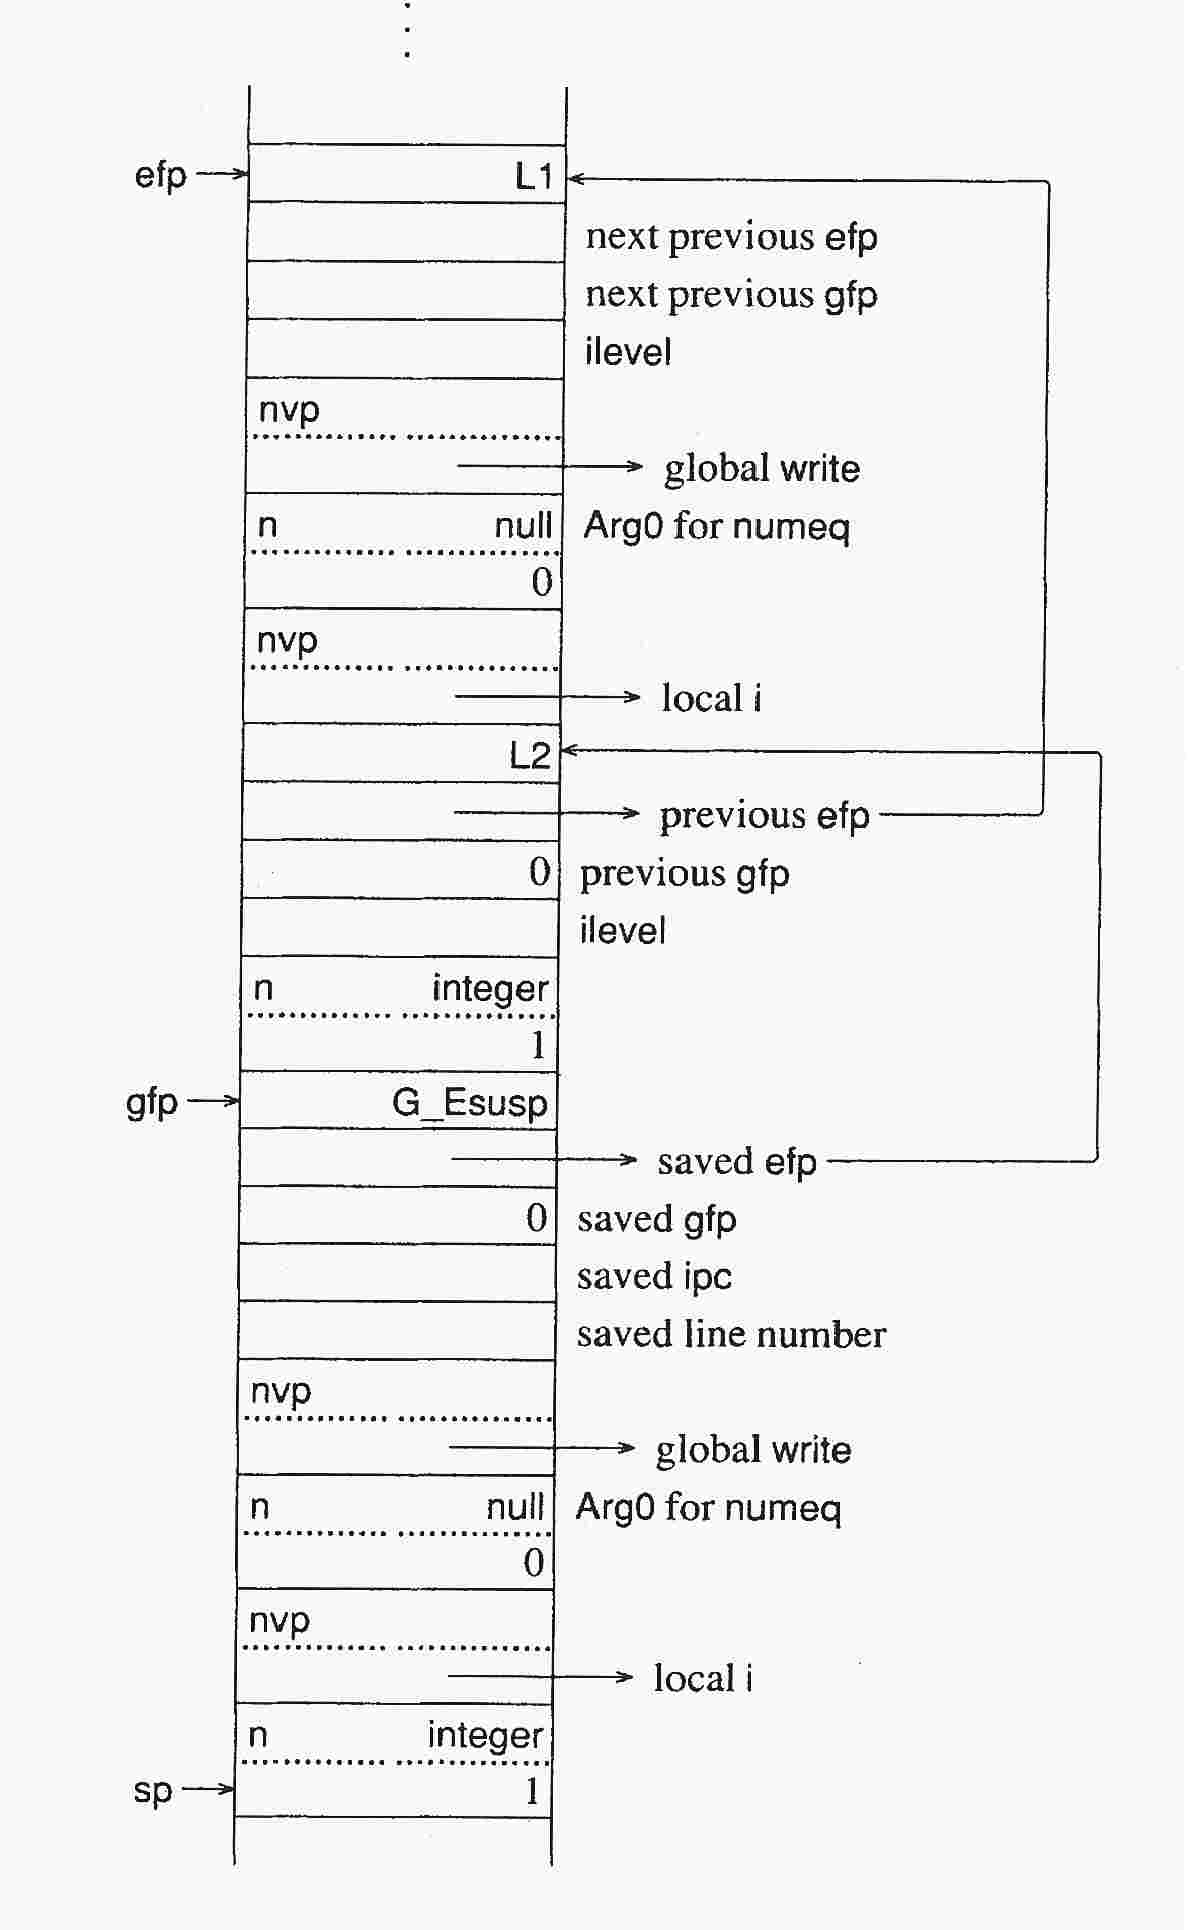
\includegraphics[width=4.0602in,height=6.4457in]{ib-img/ib-img071.jpg} 


The top portion of the stack is the same as if \textit{expr2 }had
produced a result in the absence of alternation.  However, the
generator frame marker pushed by \texttt{esusp} contains a pointer to
the alternation marker.

If another result from \textit{expr2} is needed, the generator frame
left by \texttt{esusp} is removed, restoring the stack to its state
when \textit{expr2} produced a result. If \textit{expr2} itself was a
generator that suspended, it is resumed. Otherwise, control is
transferred to \texttt{efail} and \texttt{ipc} is set to a value
corresponding to \texttt{L1}, so that \textit{expr3} is evaluated next.

\subsection[9.4.2 Repeated Alternation]{9.4.2 Repeated Alternation}

Alternation is the general model for generative control
structures. Repeated alternation, \texttt{{\textbar}}\textit{expr}, is
similar to alternation, and would be equivalent to

{\ttfamily\mdseries
\textit{\ \ expr }{\textbar} \textit{expr }{\textbar} \textit{expr }{\textbar} ...}

\noindent except for a special termination condition that causes
repeated alternation to stop if \textit{expr} does not produce a
result. Without this termination condition, an expression such as

{\ttfamily\mdseries
\ \ \ \ \ {\textbar}upto(c, s)}

\noindent would never return if \texttt{upto()} failed--expression
evaluation would vanish into a {\textquotedbl}black
hole.{\textquotedbl} Expressions that produce results at one time but
not at another also are useful. For example,

{\ttfamily\mdseries
\ \ \ \ \ {\textbar}read()}

\noindent generates the lines from the standard input file. Because of
the termination condition, this expression terminates when the end of
the input file is reached. If it vanished into a {\textquotedbl}black
hole,{\textquotedbl} it could not be used safely.

If it were not for the termination condition, the virtual machine
instructions for \texttt{{\textbar}}\textit{expr} would be

{\ttfamily\mdseries
L1:}

{\ttfamily\mdseries
\ \ \ \ \ \ mark L1}

{\ttfamily\mdseries
\ \ \ \ \ \ \textit{code for expr}}

{\ttfamily\mdseries
\ \ \ \ \ \ esusp}


The {\textquotedbl}black hole{\textquotedbl} here is evident---if
\textit{expr} fails, it is evaluated again and there is no way out.

The termination condition is handled by an instruction that changes
the failure \texttt{ipc} in the current expression marker. The actual
virtual machine instructions for \texttt{{\textbar}}\textit{expr} are

{\ttfamily\mdseries
L1:}

{\ttfamily\mdseries
\ \ \ \ \ \ mark0}

{\ttfamily\mdseries
\ \ \ \ \ \ code for expr}

{\ttfamily\mdseries
\ \ \ \ \ \ chfail\ \ L1}

{\ttfamily\mdseries
\ \ \ \ \ \ esusp}


The virtual machine instruction \texttt{mark0} pushes an expression
frame marker with a zero failure \texttt{ipc}. If a zero failure
\texttt{ipc} is encountered during failure, as illustrated by the code
for \texttt{efail} in Sec. 9.3, failure is transmitted to the
enclosing expression. If \textit{expr }produces a result, however, the
\texttt{chfail} instruction is executed. It changes the failure
\texttt{ipc} in the current expression marker to correspond to
\texttt{L1}, so that if \textit{expr }does not produce a result when
it is resumed, execution starts at the location in the icode
corresponding to \texttt{L1} again, causing another iteration of the
alternation loop. It is important to realize that \texttt{chfail} only
changes the failure \texttt{ipc} in the current expression marker on
the stack.  Subsequent execution of \texttt{mark0} creates a new
expression frame whose marker has a zero failure \texttt{ipc}.

\subsection[9.4.3 Limitation]{9.4.3 Limitation}

In the limitation control structure,

{\ttfamily\mdseries
\textit{\ \ \ expr1 }{\textbackslash} \textit{expr2}}

\noindent the normal left-to-right evaluation of Icon is reversed and
\textit{expr2 }is evaluated first. The virtual machine instructions are

{\ttfamily\mdseries
\ \ \ \ \ \ \textit{code for expr2}}

{\ttfamily\mdseries
\ \ \ \ \ \ limit}

{\ttfamily\mdseries
\ \ \ \ \ \ \textit{code for expr1}}

{\ttfamily\mdseries
\ \ \ \ \ \ lsusp}

If \textit{expr2 }succeeds, its result is on the top of the stack. The
limit instruction checks this result to be sure that it is legal---an
integer greater than or equal to zero. If it is not an integer, an
attempt is made to convert it to one. If the limit value is zero,
limit fails. Otherwise, limit creates an expression frame marker with
a zero failure \texttt{ipc} and execution continues, so that
\textit{expr1 }is evaluated in its own expression frame. During the
evaluation of \textit{expr1, }the limit value is directly below its
expression marker. For example, in

{\ttfamily\mdseries
\textit{\ \ expr1 }{\textbackslash} 10}

\noindent the stack prior to the evaluation of \textit{expr1} is

\bigskip

If \textit{expr1} produces a result, \texttt{lsusp} is executed. The
\texttt{lsusp} instruction is very similar to \texttt{esusp}. Before
producing a generator frame, however, \texttt{lsusp} decrements the
limit value. If it becomes zero, the expression frame for
\textit{expr1} is removed, the C stack is unwound, and the last value
it produced is placed on the stack in place of the limit
value. Otherwise, it copies the portion of the interpreter stack
between the end of the last expression or generator frame marker and
the limit value to the top of the stack. Note that no generator frame
is needed.

\section[9.5 Iteration]{9.5 Iteration}

The difference between evaluation and resumption in a loop is
illustrated by the virtual machine instructions for a conventional
loop

{\ttfamily\mdseries
\ \ \ while \textit{expr1 }do \textit{expr2}}

and the iteration control structure

{\ttfamily\mdseries
\ \ \ every \textit{expr1 }do \textit{expr2}}

The instructions for \texttt{while-do} are

{\ttfamily
L1:}

{\ttfamily
\ \ mark0}

{\ttfamily
\textit{\ \ code for expr1\newline
\ \ }unmark}

{\ttfamily
\ \ mark L1\newline
\ \ \textit{code for expr2\newline
\ \ }unmark}

{\ttfamily
\ \ goto\ \ L1}

If \textit{expr1} fails, the entire expression fails and failure is
transmitted to the enclosing expression frame because the failure
\texttt{ipc} is zero. If \textit{expr1} produces a result,
\textit{expr2} is evaluated in a separate expression frame. Whether
\textit{expr2} produces a result or not, its expression frame is
removed and execution continues at the beginning of the loop.

The instructions for \texttt{every-do} are

{\ttfamily\mdseries
\ \ mark0}

{\ttfamily\mdseries
\ \ code for expr1}

{\ttfamily\mdseries
\ \ pop}

{\ttfamily\mdseries
\ \ mark0}

{\ttfamily\mdseries
\ \ code for expr2}

{\ttfamily\mdseries
\ \ unmark}

{\ttfamily\mdseries
\ \ efail}


If \textit{expr1} fails, the entire expression fails and failure is
transmitted to the enclosing expression frame as in the case of
\texttt{while-do}. If \textit{expr1} produces a result, it is
discarded by the \texttt{pop} instruction, since this result is not
used in any subsequent computation. The expression frame for
\textit{expr1} is not removed, however, and \textit{expr2} is
evaluated in its own expression frame within the expression frame for
\textit{expr1} (unlike the case for the while loop). If \textit{expr2}
produces a result, its expression frame is removed and \texttt{efail}
is executed. If \textit{expr2} fails, it transmits failure to the
enclosing expression frame, which is the expression frame for
\textit{expr1}. If \textit{expr2} produces a result, \texttt{efail}
causes failure in the expression frame for \textit{expr1}. Thus, the
effect is the same, whether or not \textit{expr2} produces a
result. All results are produced simply by forcing failure.

If the expression frame for \textit{expr1} contains a generator frame,
which is the case if \textit{expr1} suspended, evaluation is resumed
accordingly, so that \textit{expr1} can produce another result. If
\textit{expr1} simply produces a result instead of suspending, there
is no generator frame, \texttt{efail} removes its expression frame,
and failure is transmitted to the enclosing expression frame.


\section[9.6 String Scanning]{9.6 String Scanning}

String scanning is one of the most useful operations in Icon. Its
implementation, however, is comparatively simple.  There is no special
expression-evaluation mechanism associated with string scanning
\textit{per se}; all {\textquotedbl}pattern matching{\textquotedbl}
follows naturally from goal-directed evaluation.

The string-scanning keywords, \texttt{\&subject} and \texttt{\&pos}
must be handled properly, however. These keywords have global scope
with respect to procedure invocation, but they are maintained in a
stack-like fashion with respect to string-scanning expressions.

The expression

{\ttfamily\mdseries
\textit{\ \ expr1 }? \textit{expr2}}

\noindent is a control structure, not an operation, since, by
definition, the arguments for ar operation are evaluated before the
operation is performed. This form of evaluation does not work for
string scanning, since after \textit{expr1} is evaluated, but before
\textit{expr2} is evaluated, the previous values of \texttt{\&subject}
and \texttt{\&pos} must be saved and new ones
established. Furthermore, when string scanning is finished, the old
values of \texttt{\&subject} and \texttt{\&pos} must be restored. In
addition, if string scanning succeeds, the values of these keywords at
the time string scanning produces a result must be saved so that they
can be restored if the string-scanning operation is resumed to produce
another result.

The virtual machine instructions for

{\ttfamily\mdseries
\textit{\ \ expr1 }? \textit{expr2}}

are

{\ttfamily\mdseries
\ \ code for expr1}

{\ttfamily\mdseries
\ \ bscan}

{\ttfamily\mdseries
\ \ code for expr2}

{\ttfamily\mdseries
\ \ escan}

If \textit{expr1} succeeds, it leaves a result on the top of the
stack. The \texttt{bscan} instruction assures that this value is a
string, performing a conversion if necessary. Otherwise, the old
values of \texttt{\&subject} and \texttt{\&pos} are pushed on the
stack, the value of \texttt{\&subject} is set to the (possibly
converted) one produced by \textit{expr1}, and \texttt{\&pos} is set
to 1.


The \texttt{bscan} instruction then suspends. This is necessary in
case \textit{expr2} fails, so that \texttt{bscan} can get control
again to perform data backtracking, restoring the previous values of
\texttt{\&subject} and \texttt{\&pos} from the stack where they were
saved.


If \textit{expr2} succeeds, the \texttt{escan} instruction copies the
descriptor on the top of the stack to its Arg0 position, overwriting
the result produced by \textit{expr2}. It then exchanges the current
values of \texttt{\&subject} and \texttt{\&pos} with those saved by
\texttt{bscan} thus restoring the values of these keywords to their
values prior to the scanning expression and at the same time saving
the values they had at the time \textit{expr2} produced a result. The
\texttt{escan} instruction then suspends.

If \texttt{escan} is resumed, the values of \texttt{\&subject} and
\texttt{\&pos} are restored from the stack, restoring the situation to
what it was when \textit{expr2} produced a result. The \texttt{escan}
instruction then fails in order to force the resumption of any
suspended generators left by \textit{expr2.}

Suppose, for example, that the values of \texttt{\&subject} and
\texttt{\&pos} are \texttt{{\textquotedbl}the{\textquotedbl}} and 2
respectively, when the following expression is evaluated:

{\ttfamily\mdseries
\ \ read(f) ? move(4)}

Suppose \texttt{read(f)} produces the string
\texttt{{\textquotedbl}coconuts{\textquotedbl}}. The stack is

\ \  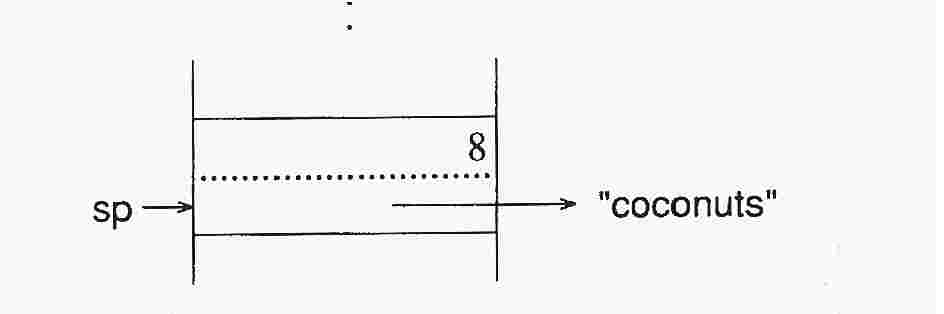
\includegraphics[width=3.2063in,height=1.048in]{ib-img/ib-img072.jpg} 

{\ttfamily\mdseries
\&subject: {\textquotedbl}the{\textquotedbl}\newline
\&pos: 2}

The \texttt{bscan} instruction is executed, pushing the current values
of \texttt{\&subject} and \texttt{\&pos}:

{\sffamily
\ \  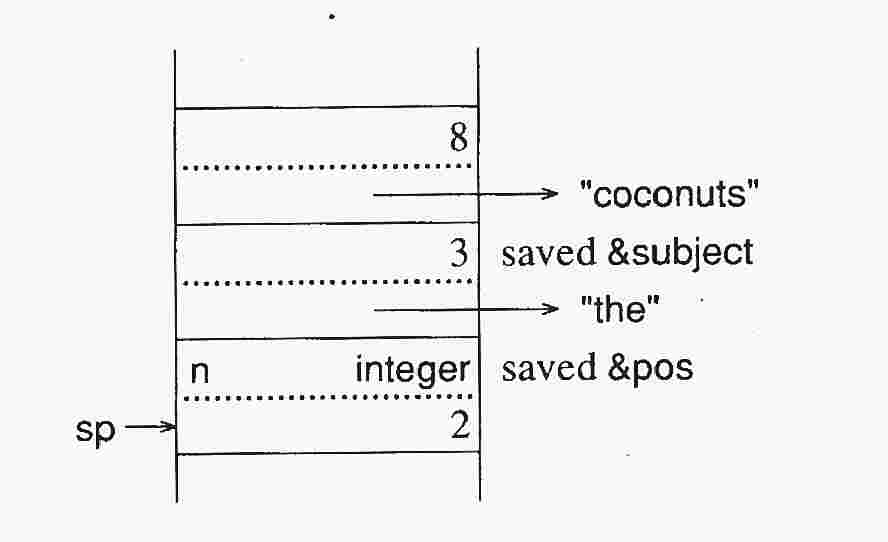
\includegraphics[width=2.9925in,height=1.8098in]{ib-img/ib-img073.jpg} }

{\ttfamily\mdseries
\&subject: {\textquotedbl}the{\textquotedbl}}

{\ttfamily\mdseries
\&pos: 2}

The \texttt{bscan} instruction sets \texttt{\&subject} to
\texttt{{\textquotedbl}coconuts{\textquotedbl}} and \texttt{\&pos} to
1. The \texttt{bscan} instruction then suspends and \texttt{move(4)}
is evaluated. It suspends, and the top I

\ \  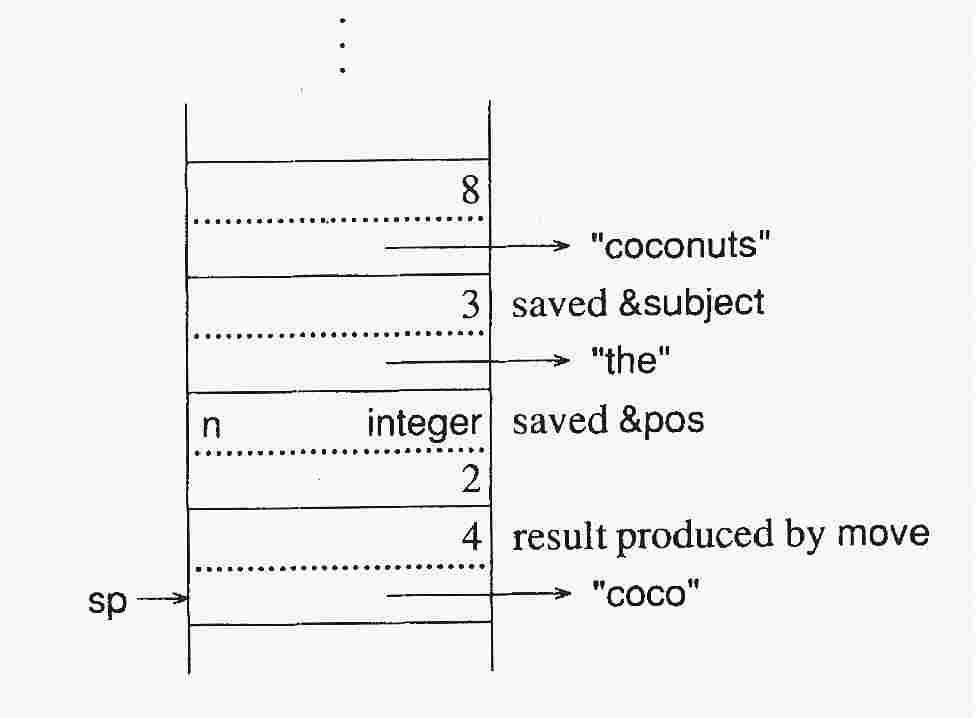
\includegraphics[width=3.3134in,height=2.398in]{ib-img/ib-img074.jpg} 

{\ttfamily\mdseries
\&subject: {\textquotedbl}coconuts{\textquotedbl}\newline
\&pos: 5}

The \texttt{escan} instruction is executed next. It copies the
descriptor on the top of the stack to replace the result produced by
\textit{expr2. }It then exchanges the current values of
\texttt{\&subject} and \texttt{\&pos} with those on the stack:

\ \  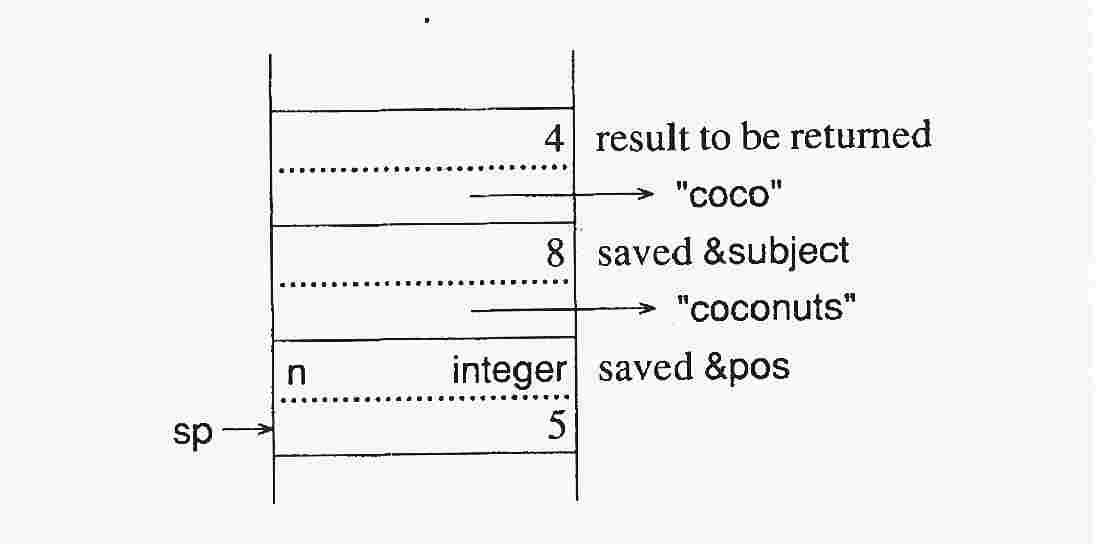
\includegraphics[width=3.7402in,height=1.8161in]{ib-img/ib-img075.jpg} 

{\ttfamily\mdseries
\&subject: {\textquotedbl}the{\textquotedbl}\newline
\&pos: 2}

The \texttt{escan} instruction then suspends, building a generator
frame. The result of \textit{expr2} is placed on the top of the stack,
becoming the result of the entire scanning expression.

\ \  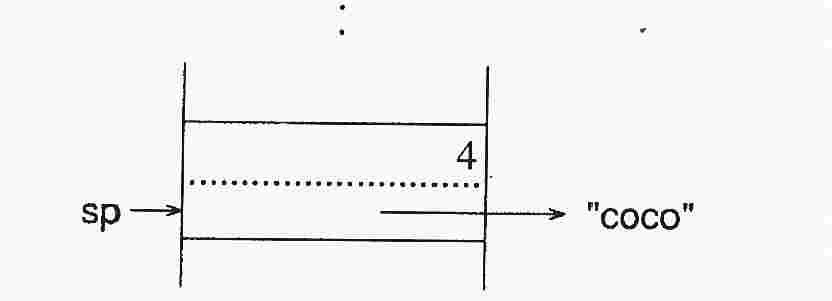
\includegraphics[width=2.778in,height=1.0043in]{ib-img/ib-img076.jpg} 

Since \texttt{escan} suspends, the saved values of \texttt{\&subject}
and \texttt{\&pos} are preserved in a generator frame on the stack
until \texttt{escan} is resumed or until the current expression frame
is removed.

\textsc{Retrospective}: The implementation of expression evaluation in
Icon focuses on the concept of an expression frame within which
control backtracking can occur. Bounded expressions, for example, are
represented on the stack by expression frames, which confine
backtracking.

In the absence of generators, failure simply results in the removal of
the current expression frame and transfer to a new location in the
icode, bypassing instructions that otherwise would have been executed.

State information must be saved when a generator suspends, so that its
evaluation can be resumed. This information is preserved in a
generator frame within the current expression frame. Generator frames
are linked together in a last-in, first-out fashion. Goal-directed
evaluation is a natural consequence of resuming the most recently
suspended generator when an expression fails, instead of simply
removing the current expression frame.

String scanning involves saving and restoring the values of
\texttt{\&subject} and \texttt{\&pos}. This is somewhat complicated,
since scanning expressions can suspend and be resumed, but string
scanning itself introduces nothing new into expression evaluation:
generators and goal-directed evaluation provide {\textquotedbl}pattern
matching.{\textquotedbl}

\bigskip

\noindent\textbf{EXERCISES}

\textbf{9.1} Circle all the bounded expressions in the following segments of code:

{\ttfamily\mdseries
\ \ \ while line := read() do}

{\ttfamily\mdseries
\ \ \ \ \ \ if *line = i then write(line)}


\bigskip

{\ttfamily\mdseries
\ \ \ if (i = find(s1,s2)) \& (j = find(s1,s3)) then \{}

{\ttfamily\mdseries
\ \ \ \ \ \ write(i)}

{\ttfamily\mdseries
\ \ \ \ \ \ write(j)}

{\ttfamily\mdseries
\ \ \ \ \ \ \}}


\bigskip

{\ttfamily\mdseries
\ \ \ line ? while write(move(1)) do}

{\ttfamily\mdseries
\ \ \ \ \ \ \ \ \ move(1)}


\textbf{9.2} Describe the effect of nested generators and generators in mutual
evaluation on the interpreter level.

\textbf{9.3} Consider a hypothetical control structure called
\textit{exclusive alternation} that is the same as regular
alternation, except that if the first argument produces least one
result, the results from the second argument are not produced. Show
the virtual machine instructions that should be generated for
exclusive alternation.

\textbf{9.4} The expression \texttt{read(f)} is an example of an expression
that may produce result at one time and fail at another. This is
possible because of a side effect of evaluating it---changing the
position in the file f. Give an example of an expression that may fail
at one time and produce a result at a subsequent time.

\textbf{9.5} There are potential ``black holes'' in
the expression-evaluation mechanism of Icon, despite the termination
condition for repeated alternation. Give an example of one.

\textbf{9.6} The expression frame marker produced by limit makes it easy to
locate the limitation counter. Show how the counter could be located
without the marker.

\textbf{9.7} Suppose that the virtual machine instructions for

{\ttfamily\mdseries
\ \ \ every \textit{expr1} do \textit{expr2}}

\noindent did not pop the result produced by \textit{expr1}. What
effect would this have?

\textbf{9.8} The virtual machine instructions for

{\ttfamily\mdseries
\ \ \ every expr}

are

{\ttfamily\mdseries
\ \ \ mark0}

{\ttfamily\mdseries
\ \ \ \textit{code for expr}}

{\ttfamily\mdseries
\ \ \ pop}

{\ttfamily\mdseries
\ \ \ efail}

\noindent so that failure causes \textit{expr} to be resumed. The
keyword \texttt{\&fail} also fails, so that the virtual machine
instructions for

{\ttfamily\mdseries
\textit{\ \ \ expr }\& \&fail}

are

{\ttfamily\mdseries
\ \ \ \textit{code for expr}}

{\ttfamily\mdseries
\ \ \ efail}

It is sometimes claimed that these two expressions are equivalent. If
this were so, the shorter virtual machine instruction sequence for the
second expression could be used for the first expression. Explain why
the two expressions are not equivalent, in general, and give an
example in which they are different.

\textbf{9.9} Diagram the states of the stack for the example given in
Sec. 9.6, showing all generator frames.

\textbf{9.10} Show the successive stack states for the evaluation of the
following expressions, assuming that the values of \texttt{\&subject}
and \texttt{\&pos} are \texttt{"the"} and
2 respectively, and that \texttt{read()} produces
\texttt{"coconuts"} in each case:

\ \ (a) read(f) ? move(10)\newline
\ \ (b) (read(f) ? move(4)) ? move(2)\newline
\ \ (c) read(f) ? (move(4) ? move(2))\newline
\ \ (d) (read(f) ? move(4)) ? move(10)\newline
\ \ (e) (read(f) ? move(4 {\textbar} 6)) ? move(5)\newline
\ \ (f) (read(f) ? move(4)) \& (read(f) \& move(10))

\textbf{9.11} Write Icon procedures to emulate string
scanning. \textit{Hint:} consider the virtual machine instructions for

{\ttfamily\mdseries
\textit{\ \ expr1 }? \textit{eXpr2}}
